
%----------------------------------------------------------------------------------------
%	PACKAGES AND DOCUMENT CONFIGURATIONS
%----------------------------------------------------------------------------------------

\documentclass[12pt,a4paper]{article}

\usepackage[version=3]{mhchem} % Package for chemical equation typesetting
\usepackage{siunitx} % Provides the \SI{}{} and \si{} command for typesetting SI units
\usepackage{graphicx} % Required for the inclusion of images
\usepackage{natbib} % Required to change bibliography style to APA
\usepackage{amsmath} % Required for some math elements 
\usepackage{geometry}
\usepackage{enumerate}
\usepackage{textcomp}
\usepackage{siunitx}
\usepackage{hhline}
\usepackage{caption}
\usepackage{booktabs}
\usepackage{multirow}
\usepackage{float}
\usepackage{longtable}
\usepackage{pdfpages}

\includepdfset{pagecommand={\thispagestyle{fancy}}}%page number for pdf

\renewcommand{\labelenumi}{\alph{enumi}.} % Make numbering in the enumerate environment by letter rather than number (e.g. section 6)
\geometry{left=1cm,right=1cm,top=1cm,bottom=1.5cm}

%\usepackage{times} % Uncomment to use the Times New Roman font

%----------------------------------------------------------------------------------------
%	DOCUMENT INFORMATION
%----------------------------------------------------------------------------------------


\begin{document}
\thispagestyle{empty}
\begin{center}

    \begin{description}
        \item[] 
        \item[]
        \item[]
    \end{description}
    

\Large{ \textsc{\newline\rule{14.3cm}{0.05em}\newline\\UM-SJTU Joint Institute\\Physics Laboratory\\(Vp141)\\}}
\rule{14.3cm}{0.05em}
\LARGE{\textsc{\newline\newline\newline\newline\newline\\
Laboratory Report\\}}
\Large{\textsc{  \\ Exercise 3  \\ Simple Harmonic Motion:
\\Oscillations in Mechanical Systems\\
} }

\end{center}

\begin{description}
    \item[] 
    \item[] 
    \item[] 
    \item[] 
    \item[] 
    \item[]
    \item[]
    \item[]
    \item[]\textbf{\qquad \qquad Name: Han Yibei \qquad ID:519370910123   \qquad    Group:11     }
    \item[]\qquad \qquad Name: Lu Xinyi \qquad ID:519370910122   \qquad    Group:11  
    \item[]\qquad \qquad Date: \today
\end{description}

\newpage
\setcounter{page}{1}

%----------------------------------------------------------------------------------------
%	SECTION 1
%----------------------------------------------------------------------------------------

\section{Introduction}
The objective of this experiment is to study properties of a simple harmonic oscillation. We will first apply Hooke’s law to find out the spring constant. Then, we will do several control experiments on the air track to study the relationship between the oscillation period and the mass, the period and the amplitude, and the maximum speed and the amplitude.

\section{Theoratical background}
\subsection{Hooke's Law}
Within the elastic limit of deformation, the restoring force of the spring has the direction opposite to the deformation and its magnitude is directly proportional to the distance. Hooke’s Law can be expressed by:
\begin{equation}
    F_x=kx
\end{equation}
where k is the spring constant, $F_x$ is known as the restoring force and can be found using the Jolly balance.
\subsection{Equation of Motion of the Simple Harmonic Oscillator}
An object with mass M is placed on an air track which serves to eliminate the frictional force, as shown in Fig.\ref{masssystem}. 

The two ends of the object are fixed to the air track using two springs whose spring constants are k1 and k2. Neglecting the masses of the springs and the damping and applying Newton’s second law, the equation of motion of the object is:s
\begin{equation}
    M\frac{d^2x}{dt^2}+(k_1+k_2)x=0\ \ \Rightarrow\ \ x(t)=A\cos{\omega_0t+\phi_0}
\end{equation}
where $\omega_0=\sqrt{(k_1+k_2)/M}$, which is the natural angular frequency of the oscillations and is determined by the parameters of the system itself. A is the amplitude and $\phi_0$ is the initial phase which is determined by initial conditions.\par 
The natural period of oscillation is:
\begin{equation}
    T=\frac{2\pi}{\omega_0}=2\pi\sqrt{\frac{M}{k_1+k_2}}\ \ \Rightarrow\ \     \frac{T^2}{m}=\frac{4\pi^2}{k_1+k_2}
\end{equation}

\subsection{Mass of the Spring}
When the mass of springs cannot be ignored, we consider the effective mass of the spring, which is 1/3 of the actual mass of the spring. The oscillator with object of mass M and spring of effective mass $m_0$ has the angular frequency:

\begin{equation}
    \omega_0=\sqrt{\frac{k_1+k_2}{M+m_0}}
\end{equation}

\subsection{Mechanical Energy in Harmonic Motion}
The elastic potential energy of the spring-mass system is $U=kx^2/2$ and the kinetic energy of it is $K=mv^2/2$.\par 
The speed of the mass is maximized at the equilibrium position x=0, where the total mechanical energy equals to maximum kinetic energy. At maximum displacement, the mass has no speed and has maximum potential energy as the total mechanical energy. Therefore, as there are only conservative forces, Kmax = Umax, and we get:
\begin{equation}
    k=\frac{mv^2_{max}}{A^2}
\end{equation}

Other things needed: $\Delta x=(x_{in}+x_{out})/2$, $v_{max}=\Delta x/\Delta t$. Where $x_{in}$ is the distance within the two legs of the U shape shutter and $x_{out}$ is the outer distance. $\Delta t$ is the time it takes to travel from one leg of the U shape shutter to the other, which is measured by the timer.


\section{Experimental setup}
The measurement equipment consists of: springs, Jolly balance, air track, electronic timer, electronic balance, and masses.

\subsection{Jolly balance}
The scale on the Jolly balance is used to measure the deformation of the spring, from which we can calculate the spring constant. It's shown in Fig.\ref{jolly}.

First, put the initial 20g mass on the bottom end of the spring, read the scale L1. Then add mass m to it and read L2. The spring constant can be found as:
$$k=\frac{mg}{L2-L1}$$\par
Read the readings onlly if the three lines coincide: the line on the mirror, the line on the glass tude and its reflection in the mirror.

\subsection{Photoelectric Measuring System}
For period measurement, we use the I-shape shutter on the moving object to block the light emitted from the photoelectric gate. Each time the light is blocked, half a period is counted.\par 
For speed measurement, we use a U-shape shutter, Fig.\ref{ushape}, so that the light is blocked twice during a pass. The time interval $\Delta t$ is measured by the timer, and we use a caliper to measure the distance $x_{in}$ and $x_{out}$  to get $\Delta_x=\frac{1}{2}(x_{in}+x_{out})$. Therefore, the instantaneous speed can be expressed by $v=\frac{\Delta_x}{\Delta_t}$.\par 

The whole setup is shown in Fig.\ref{setup}

\subsection{Device information}

\begin{table}[H]
    \centering
    \begin{tabular}{ccc}
        \hline
    Apparatus & & Precision \\\hline  
    Jolly Balance & & 0.02[mm] \\ 
    Caliper & & 0.02[mm]  \\
    Electronic balance & & 0.01[g] \\
    \multirow{2}{*}{Photoelectric measuring system} & Mode $T$   & 0.0001[s]       \\
    & Mode $S_2$ & 0.00001[s]     \\
    Air track & & 0.1[cm]       \\\hline
    \end{tabular}
    \caption{Information of Each Measurement Device}
\end{table}

\section{Measurement}
\subsection{Spring Constant}
\begin{enumerate}[1.]
    \item Adjust the Jolly balance to be vertical, and add a 20g preload to the bottom end of the spring. (Fig.\ref{jolly}) Make sure the mirror can move freely.
    \item Adjust the position of the tube to set the initial position L0 within 5.0-10.0cm and record.
    \item Add mass m1 and record L1. 
    \item Keep adding masses in order and record 7 sets of positions in total. 
    \item Use the least square method to estimate the spring constant k1.
    \item Replace spring1 with spring2 and repeat the above steps to get spring constant k2.\item Remove the preload and repeat the measurement for springs1 and 2 connected in series and calculate k3. Compare k3 with theoretical value.
\end{enumerate}

\subsection{Relation Between the Oscillation Period T and the Mass of the Oscillator M}
\subsubsection{Adjustment of the air truck}
\begin{enumerate}[1.]
    \item Adjust the air track to be horizontal. 
    \item Turn on the air pump and check if there are any holes blocked.
    \item Place the cart on the track without initial velocity and adjust the single knob until the object moves slowly back and forth in both directions.
\end{enumerate}
Caution: Don’t place anything on the track when it’s off.

\subsubsection{Horizontal air track}
\begin{enumerate}[1.]
    \item Attach the I-shape shutter to the cart and attach springs to the sides of the cart to connect it to the air track. Make sure the photoelectric gate is at the equilibrium position.
    \item Add weight m1 and let the cart oscillate about the photoelectric gate. Use a pen to release the cart and ensure that the amplitude is about 5cm. Set the timer into ‘T’ mode and it will automatically record the time of 10 oscillation periods. Record both the total time and the mass of cart. 
    \item Add weights to the cart. Repeat step 2 and take the measurements for 5 times.
    \item Plot a graph to analyze the relation between T and M.  
\end{enumerate}

\subsubsection{Inclined air track}
\begin{enumerate}[1.]
    \item Place three plastic plates under one side of the air track. Repeat steps in 4.2.2.
    \item Add three plastic plates under that side and repeat steps in 4.2.2.
    \item Plot a graph to analyze the relation between T and M. 
\end{enumerate}

\subsection{Relation Between the Oscillation Period T and the Amplitude A}
\begin{enumerate}[1.]
    \item  Fix the mass of the cart and measure the period under 6 different values of the amplitude. The recommended amplitude is 5.0/10.0/…/30.0cm.
    \item linear fit to the data and analyze the relation between T and A based on the correlation coefficient $\gamma$.
\end{enumerate}

\subsection{ Relation Between the Maximum Speed and the Amplitude}
\begin{enumerate}[1.]
    \item   Use a caliper to measure $x_{out}$ and $x_{in}$ of the U-shape shutter. Calculate the distance $\Delta x=(x_{in}+x_{out})/2$.
    \item Replace the I-shape shutter with the U-shape shutter. Set the timer into ‘S2’mode.
    \item  Measure the maximum speed of the cart under 6 different values of amplitude. The recommended amplitude is 5.0/10.0/…/30.0cm. Record the second readings of the time interval only if the two subsequent readings show the same digits to the left of the decimal point.
    \item  Apply the data to calculate the spring constant k in Eq.6 and compare this result to that in 4.1.
\end{enumerate}

\subsection{Mass measurement}
\begin{enumerate}[1.]
    \item Adjust the electronic balance every time before you use it.
    \item First weigh the cart with the I-shape shutter, then the cart with the U-shape shutter. Then measure the mass of spring1 together with spring2.
    \item Record the data only after the circular symbol on the scales display disappears.
\end{enumerate}
%----------------------------------------------------------------------------------------
%	SECTION 6
%----------------------------------------------------------------------------------------

\section{Results}

\subsection{Measurement of the spring constant}
The acceleration due to gravity given by instructor is 9.794$m/s^2$, we use the formula w=mg to calculate the weight. The detailed results are shown in Table \ref{weight}.

From Fig.\ref{constant}, we could get that for spring1, k=1.691$\pm$0.015N/m, and for spring2, k=1.58$\pm$0.12N/m.

\begin{center}
    \begin{figure}[H]
    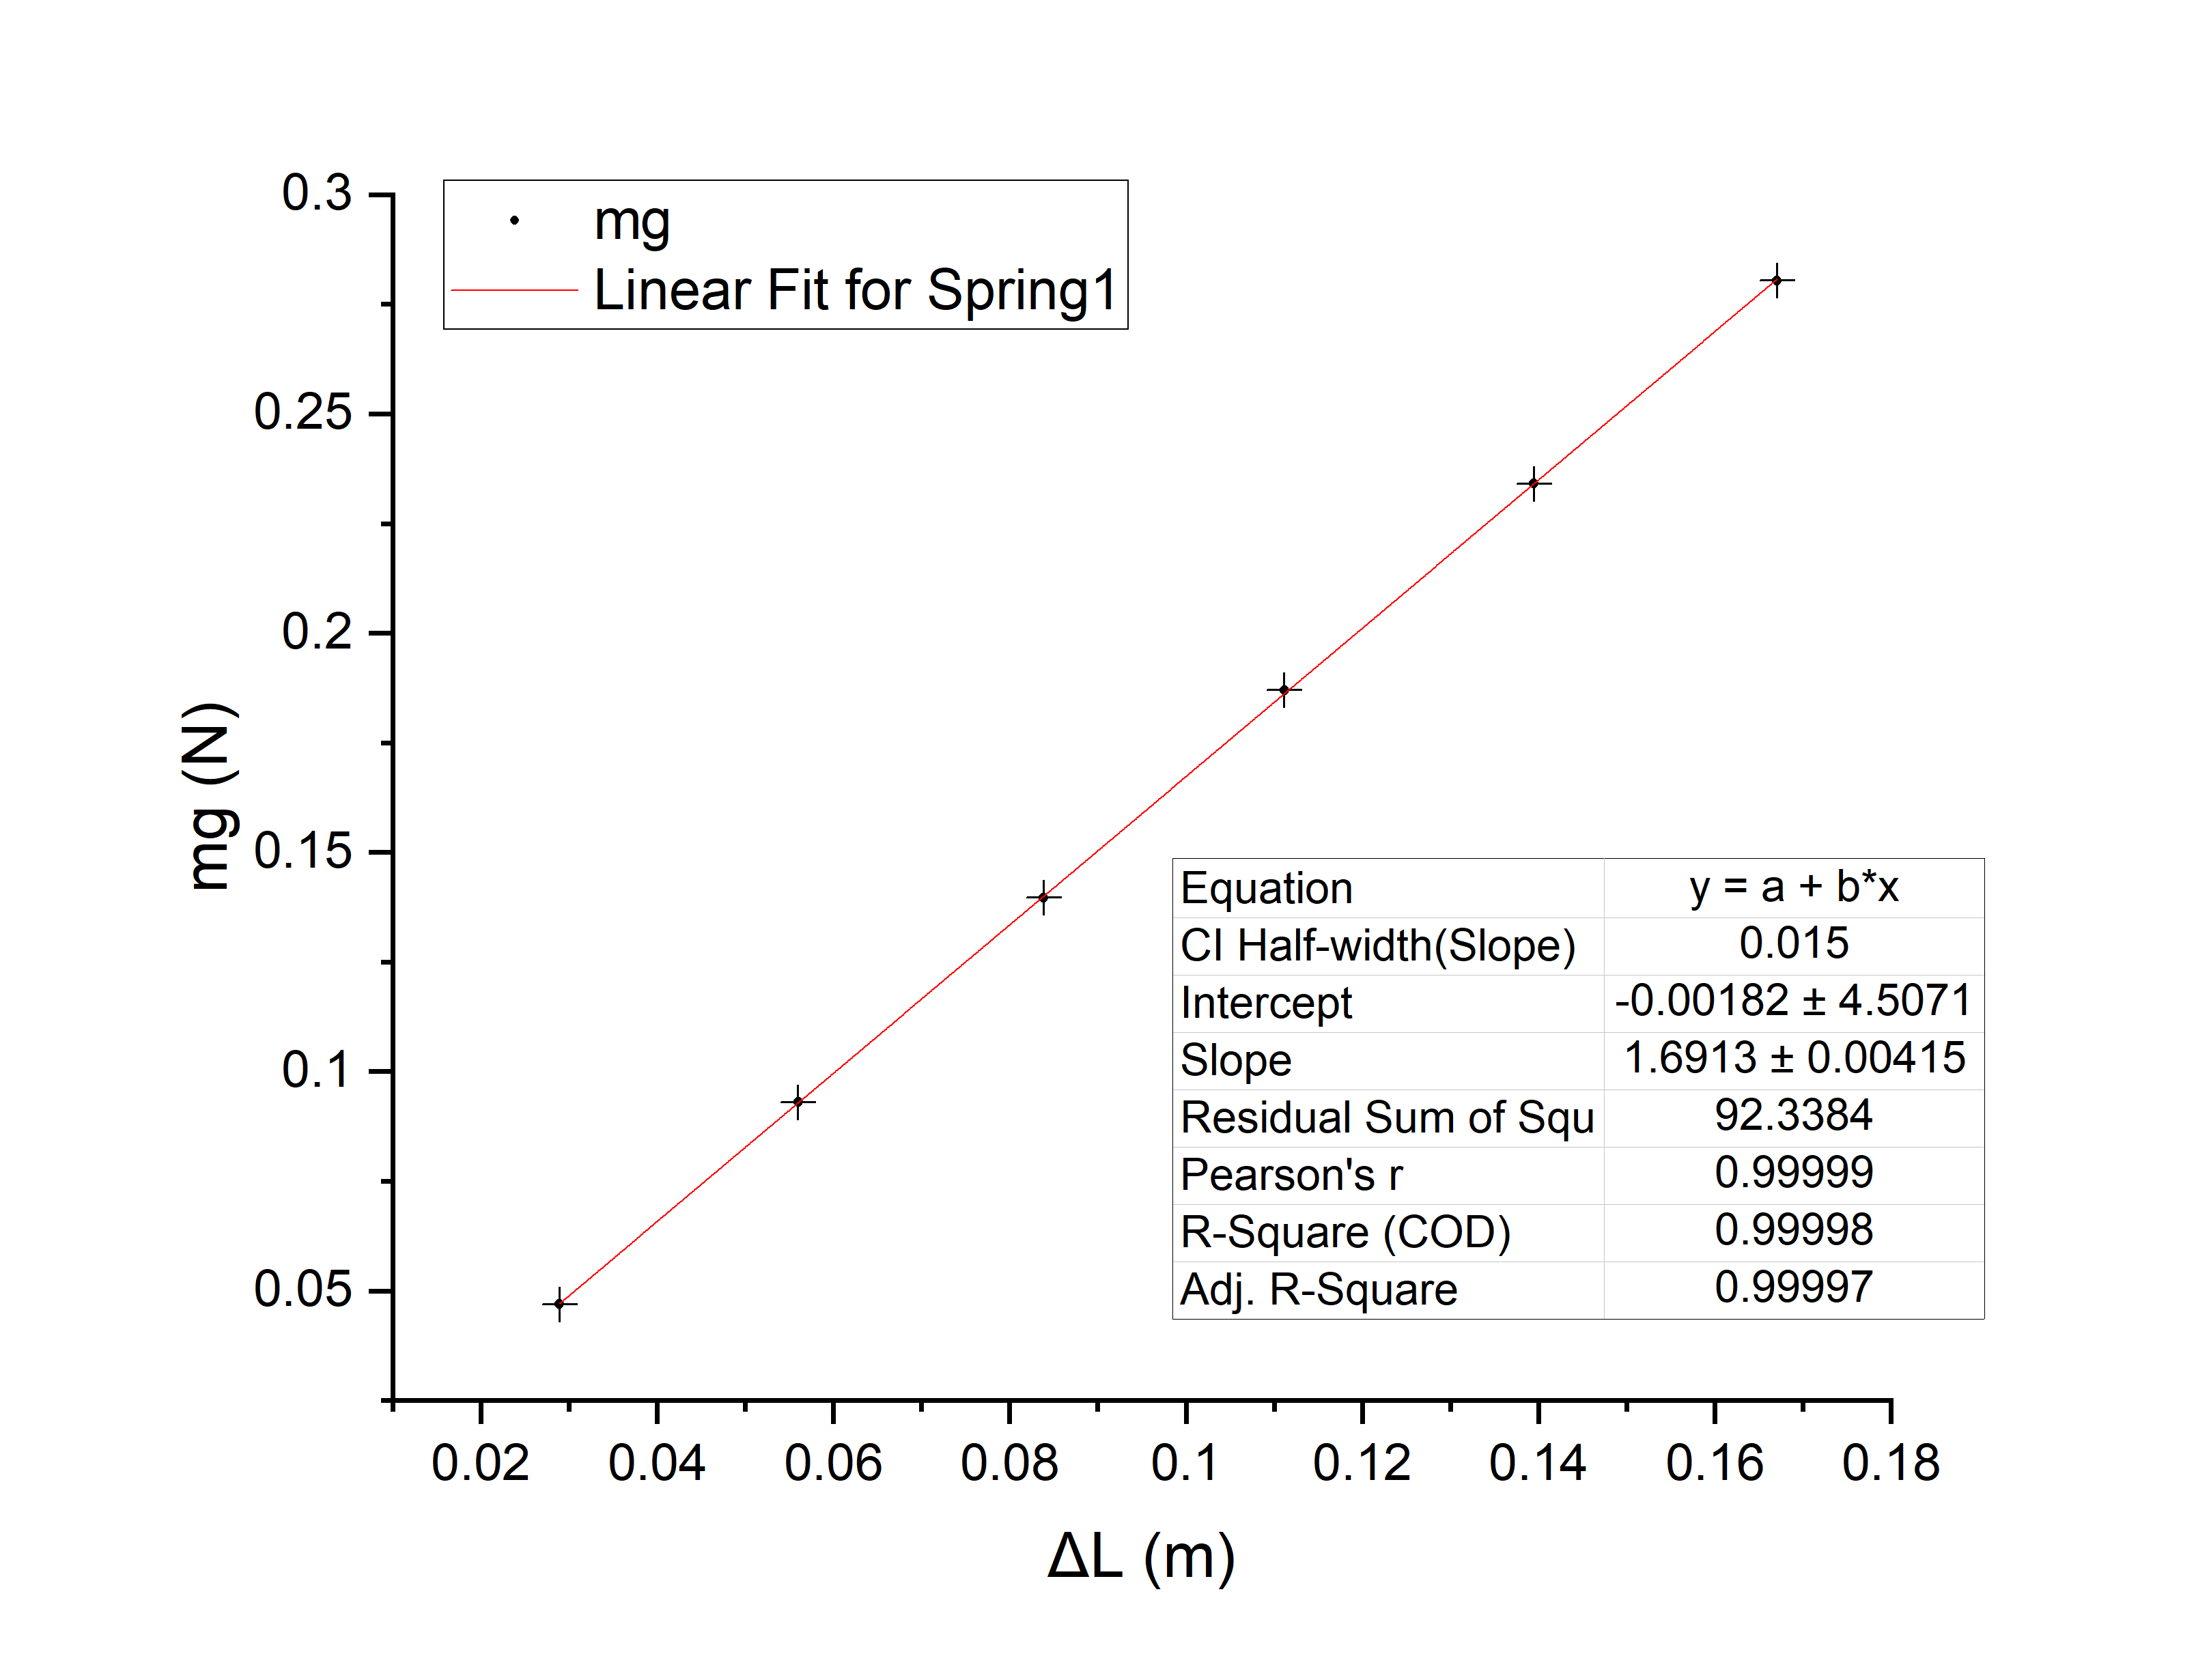
\includegraphics[scale=0.32]{k1.png}
    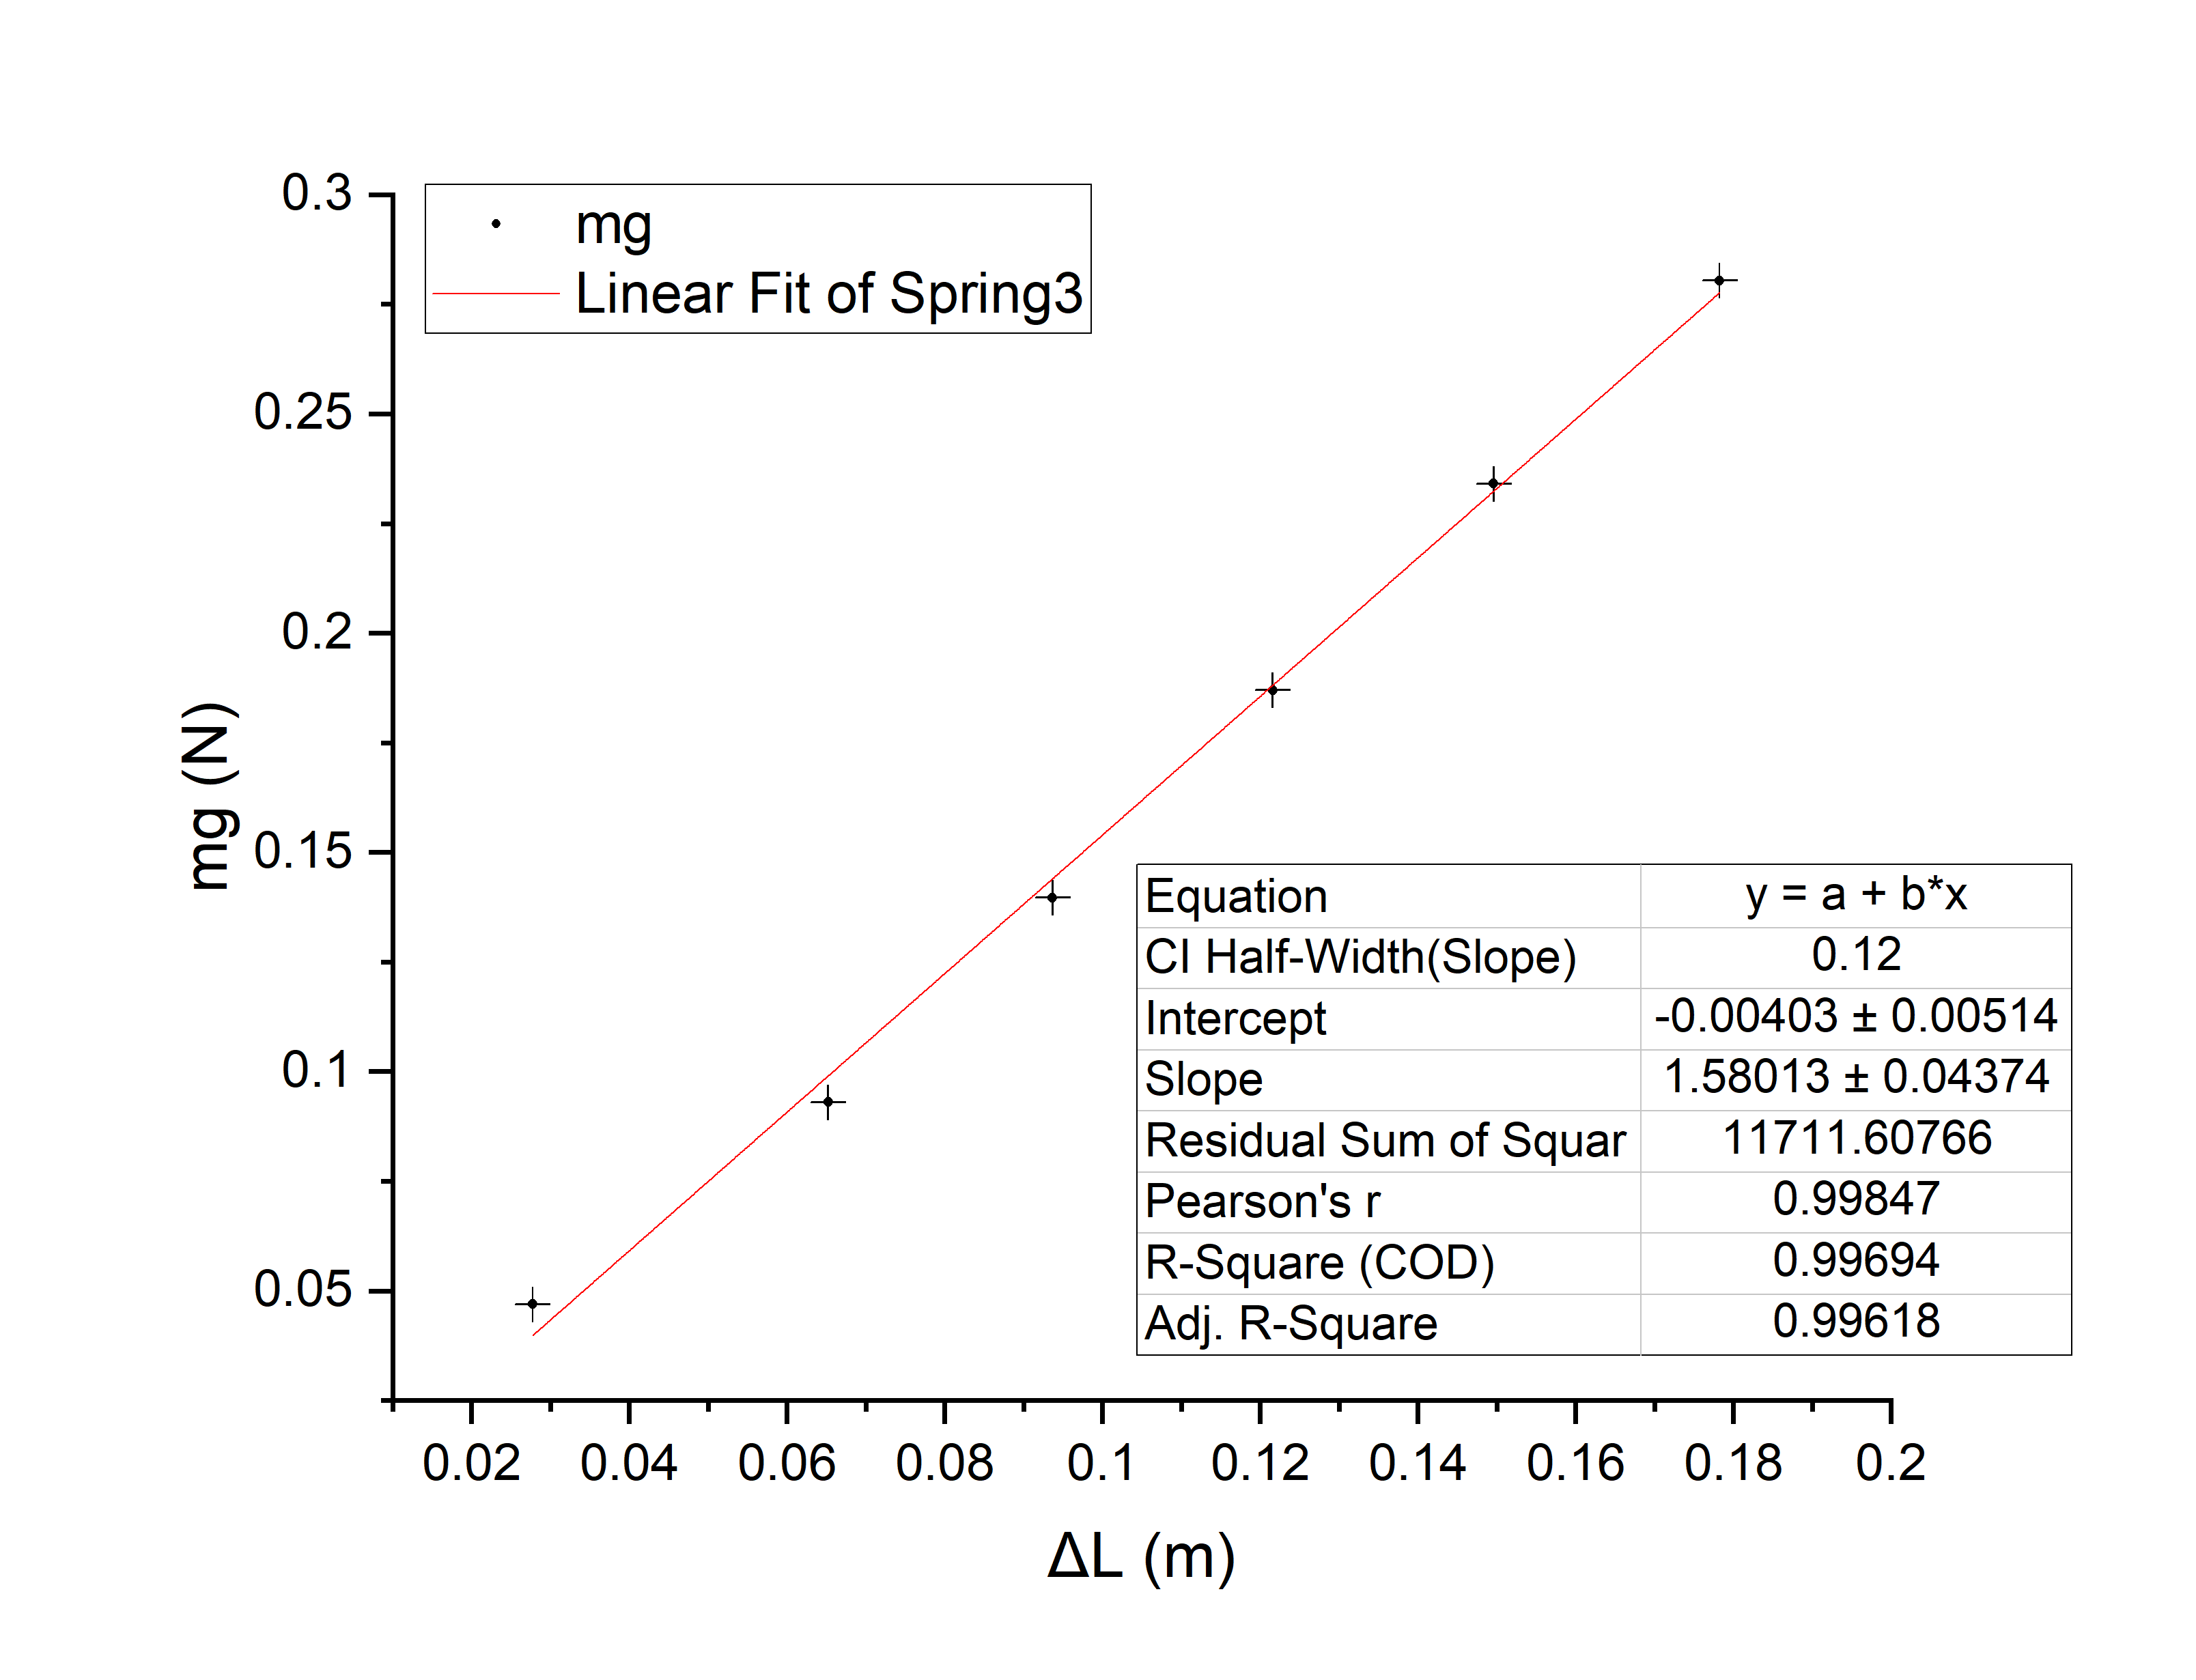
\includegraphics[scale=0.32]{k2.png}
    \caption{The linear fit figures of spring 1, 2}
    \end{figure}
    \label{constant}
\end{center}

\subsection{Relation between the Oscillation Period T and Oscillator's Mass M}
The procedure of measuring T and M are shown respectively in 4.2 and 4.5. The equivalent mass data $M_o=m_{obj}+\frac{1}{3}m_{spr1\&2}+m_{mass}$, and period data are shown in Table \ref{tsquaretable}. The uncertainty varies with T, so that the uncertainty of it is listed in table \ref{Tsquare}. Therefore,we can study the relation between T and M by linear fit $T^2$ with M, as shown in figure \ref{tsquarefigure}.
Directly from the figure, we can read the slope, which means the value and uncertainty of $\frac{T^2}{m}$, the three values are respectively:
$$11.63\pm0.08s^2/kg,~~11.59\pm0.16s^2/kg,~~11.65\pm0.03 s^2/kg$$ \par

    \begin{center}
        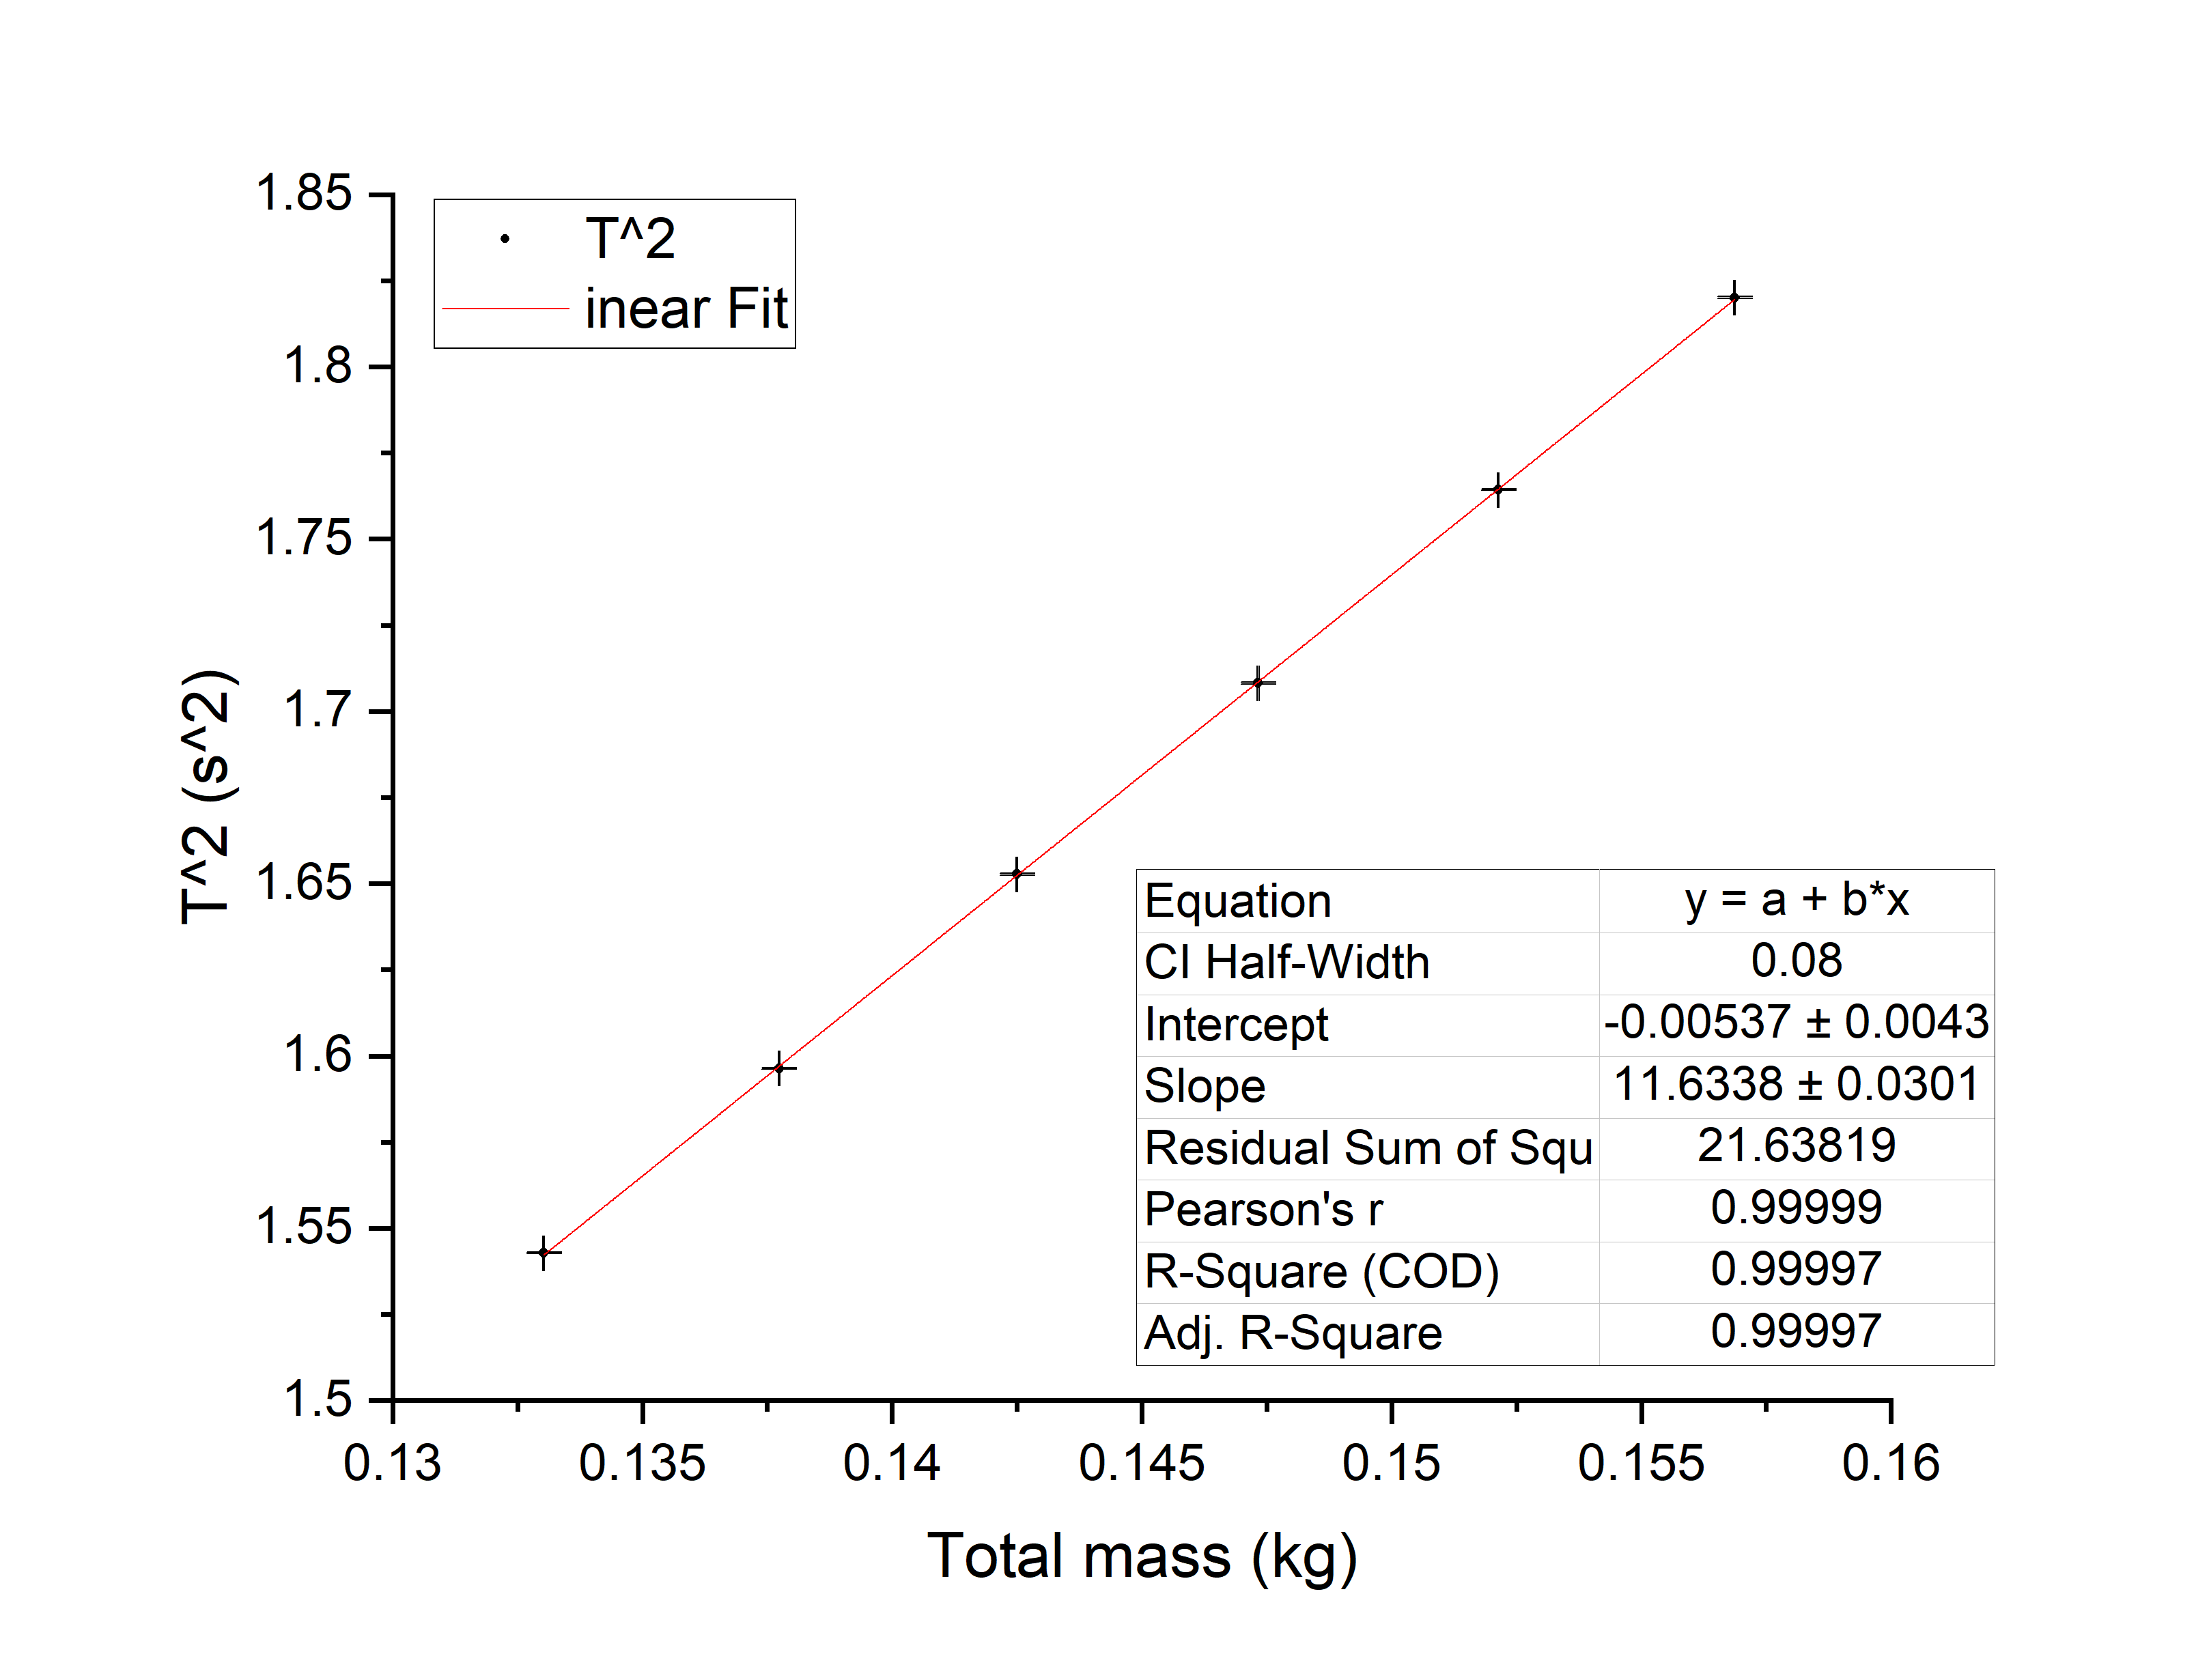
\includegraphics[scale=0.32]{horizontal.png}
        \begin{figure}[H]
                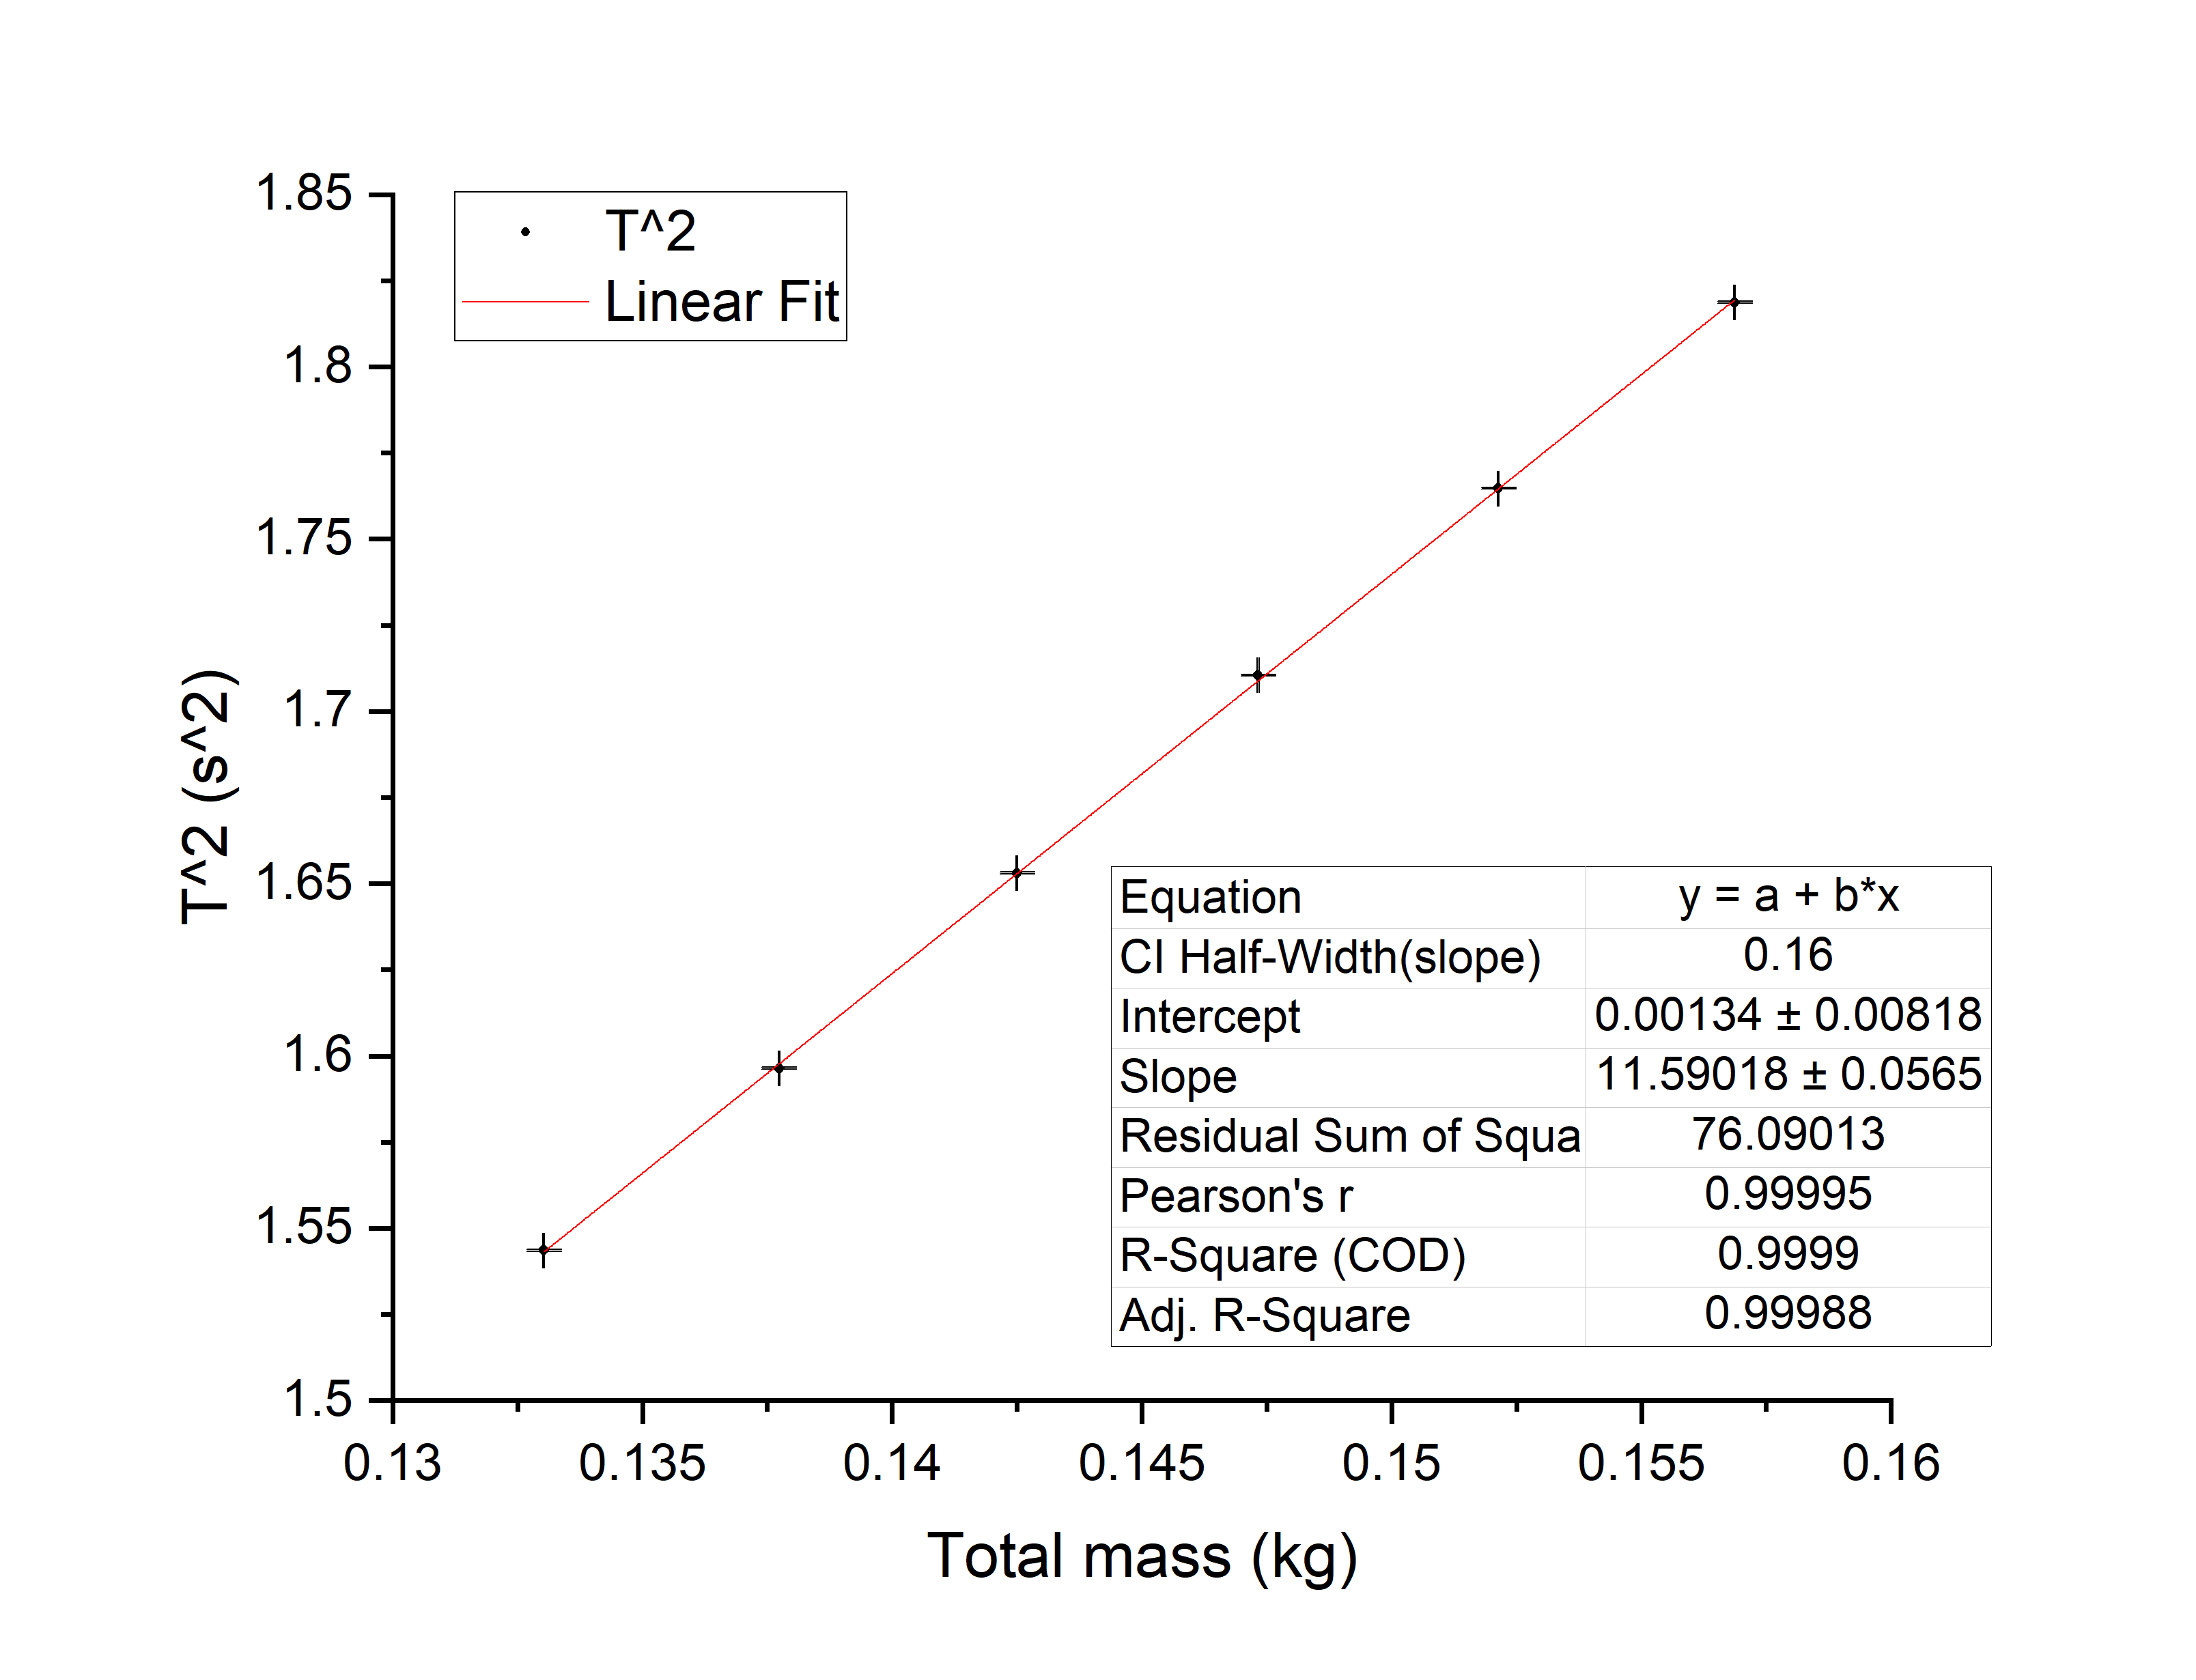
\includegraphics[scale=0.32]{incline1.png}
        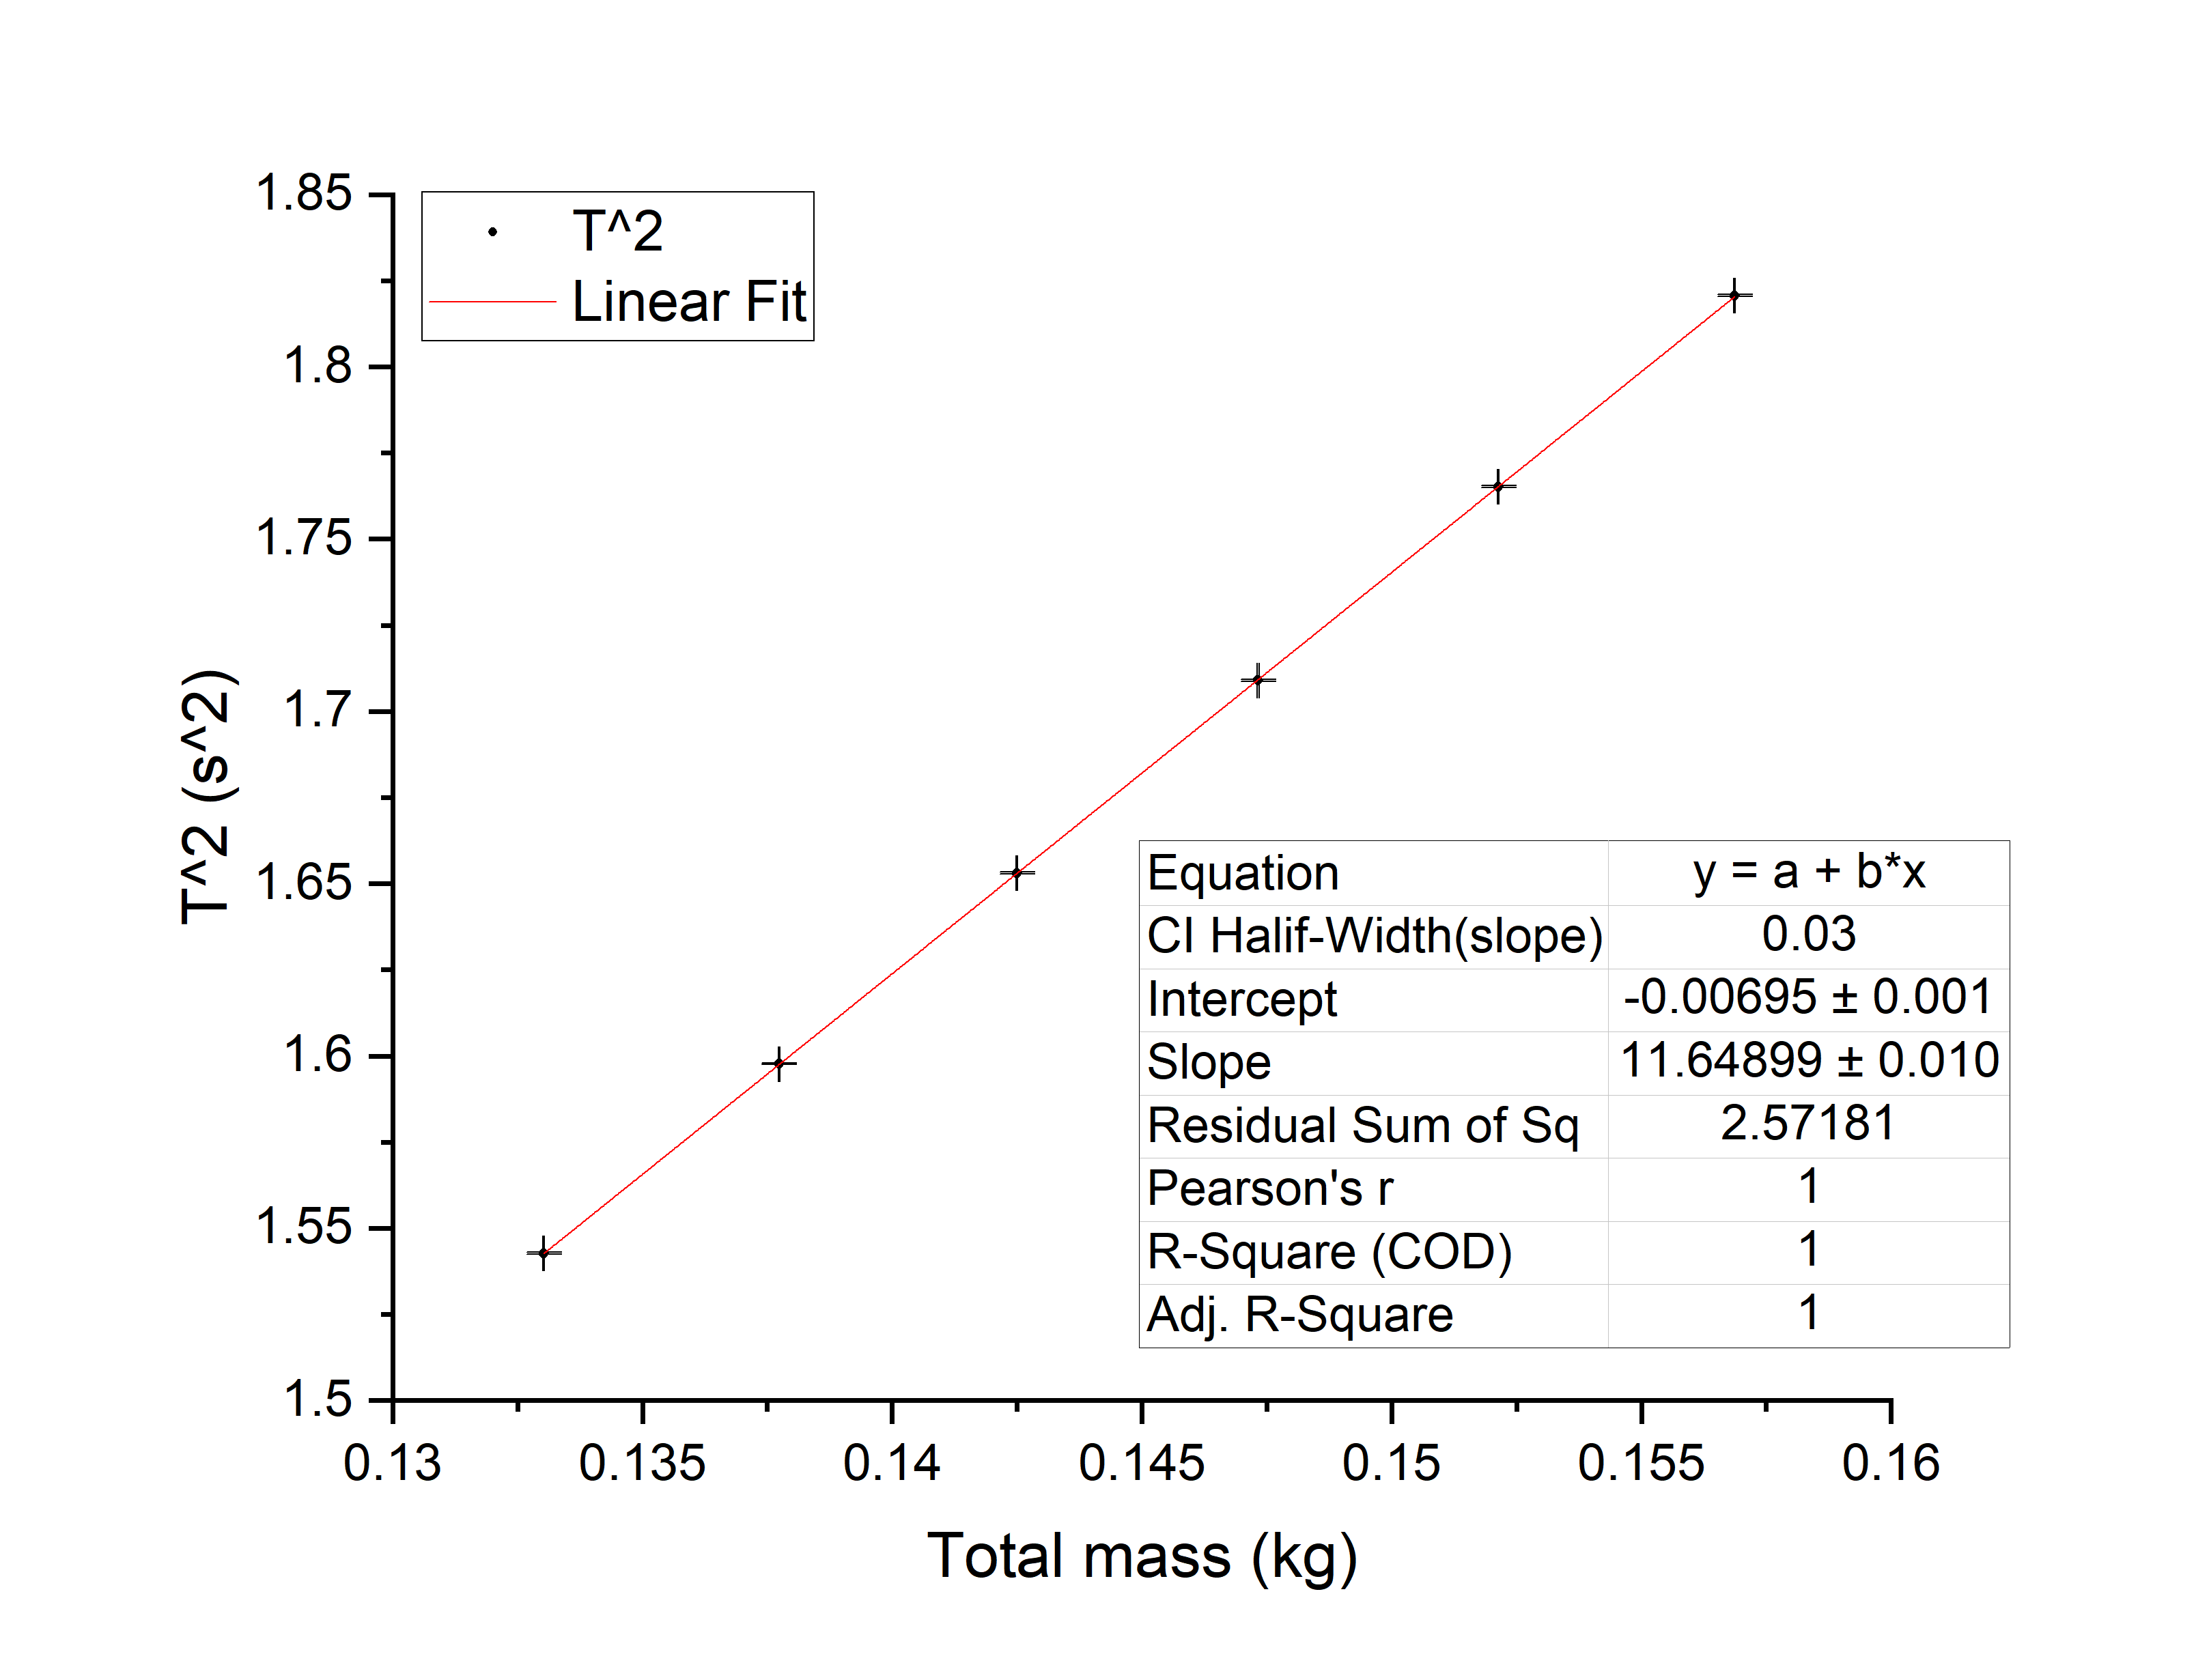
\includegraphics[scale=0.32]{incline2.png}
        \caption{Linear fit of $T^2/m$ for horizontal, incline 1, incline 2 air track.}
        \label{tsquarefigure}
        \end{figure}
    \end{center}

We know that $\frac{T^2}{m}=4\pi^2\frac{1}{k_1+k_2}$, so theoratically
$$\frac{T^2}{m}=4\pi^2\frac{1}{1.691+1.58}=12.07s^2/kg$$
Since R square is bigger than 0.75, they fit well. The relative error is 3.6\%, 4.0\%, 3.5\%.

\subsection{Relation between the Oscillation Period T and the Amplitude A}

\begin{figure}[H]
    \centering
    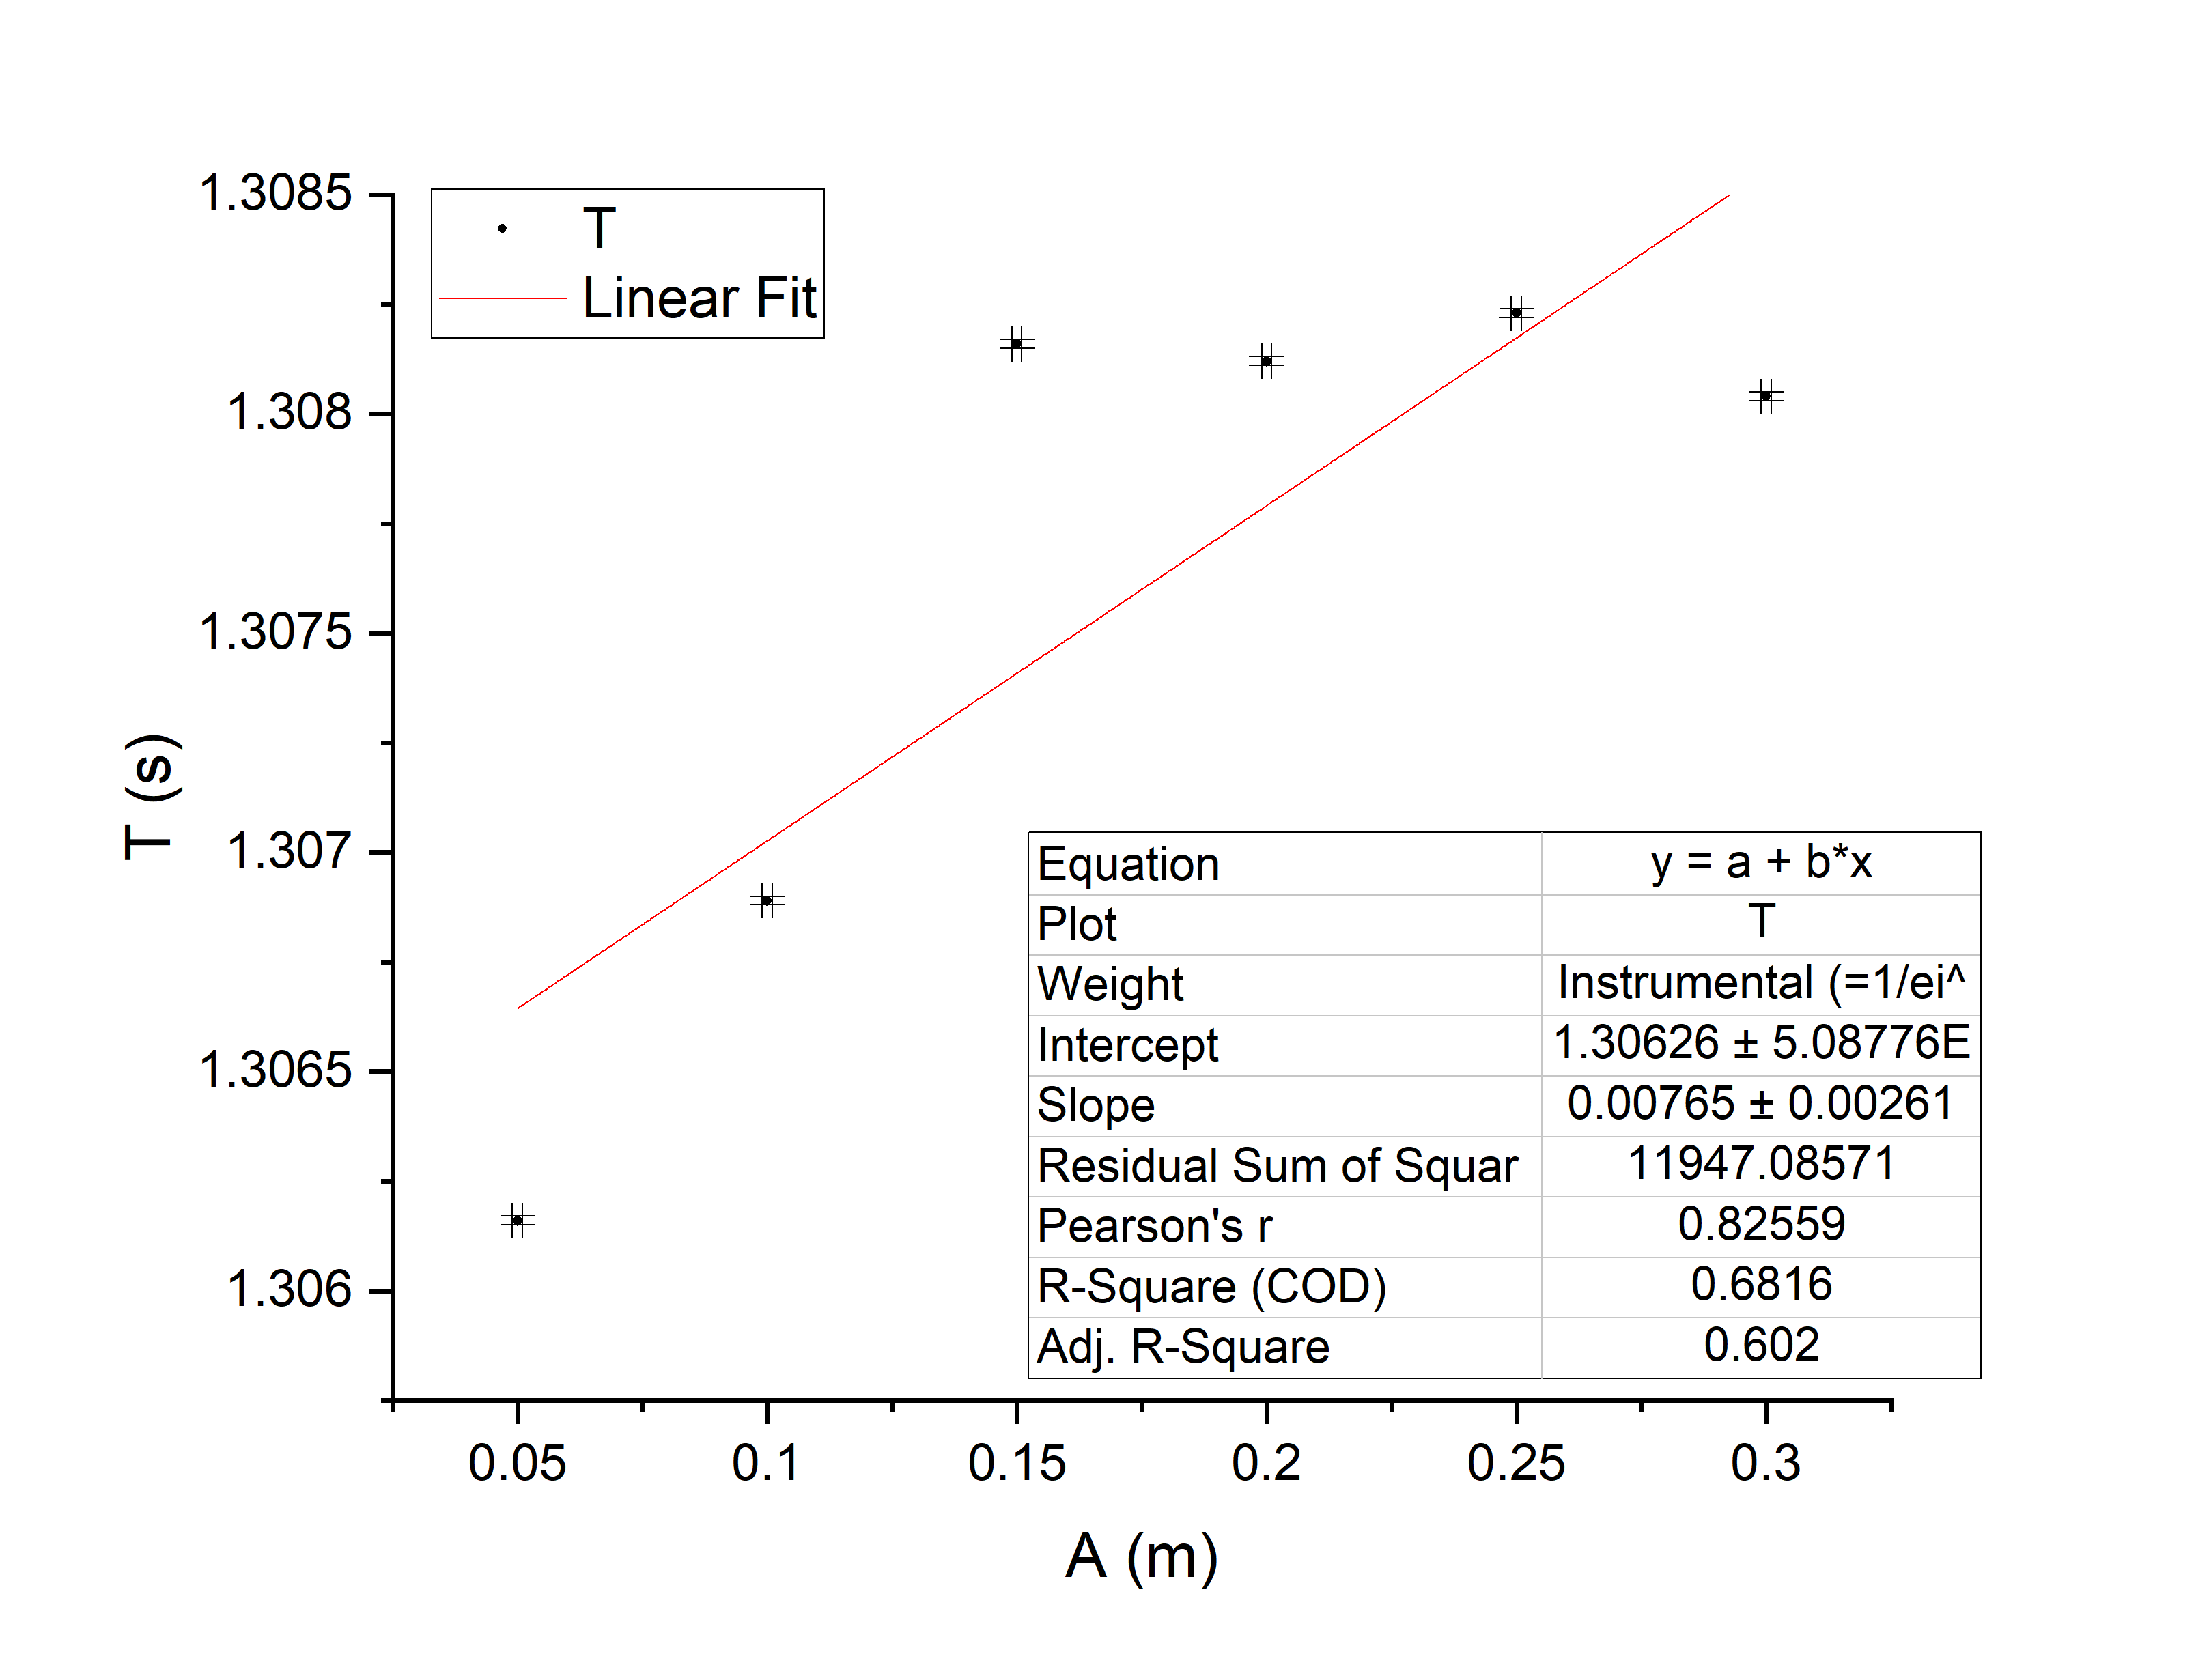
\includegraphics[scale=0.32]{amplitude.png}
    \caption{Relation between A and T}
    \label{figureAT}
\end{figure}

We apply linear fit to A and T. We can see that the slope is very close to 0, which means T is 
almost independent from A. And the R-square is smaller than 0.75. However, we find out that the Pearson’s r is 0.82, which is not small enough to indicate the independence. The possible reasons are analyzed in discussion.

\subsection{Relation between the Maximum Speed $V_{max}$  and the Amplitude A}
$$m=m_{obj,u}+\frac{1}{3}m_{spr1\&2}+m4=156.49g=0.156487\pm0.000015kg$$
Then we can calculate $m{v_{max}}^2$, the detailed data is in Table \ref{v2maxA}.

\subsubsection{Measurement of $\Delta x$}
$$\overline{x_{in}}=\sum^3_{i=1}x_{in,i}=\frac{4.44mm+4.46mm+4.44mm}{3}=4.45mm$$
$$\overline{x_{out}}=\sum^3_{i=1}x_{in,i}=\frac{15.50mm+15.54mm+15.52mm}{3}=15.52mm$$
Consider the uncertainty, we can get $\Delta x=\frac{\overline{x_{in}}+\overline{x_{out}}}{2}=9.99\pm0.03mm=0.00999\pm0.00003m$

\subsubsection{Measurement of $v_{max}$}
We apply $v_max=\frac{\Delta x}{\Delta t}$ and get the value of $v_{max}$, the detailed data is in Tabel \ref{v2maxA}.

\subsubsection{Relationship between $v_{max}$ and A}

\begin{figure}[H]
    \centering
    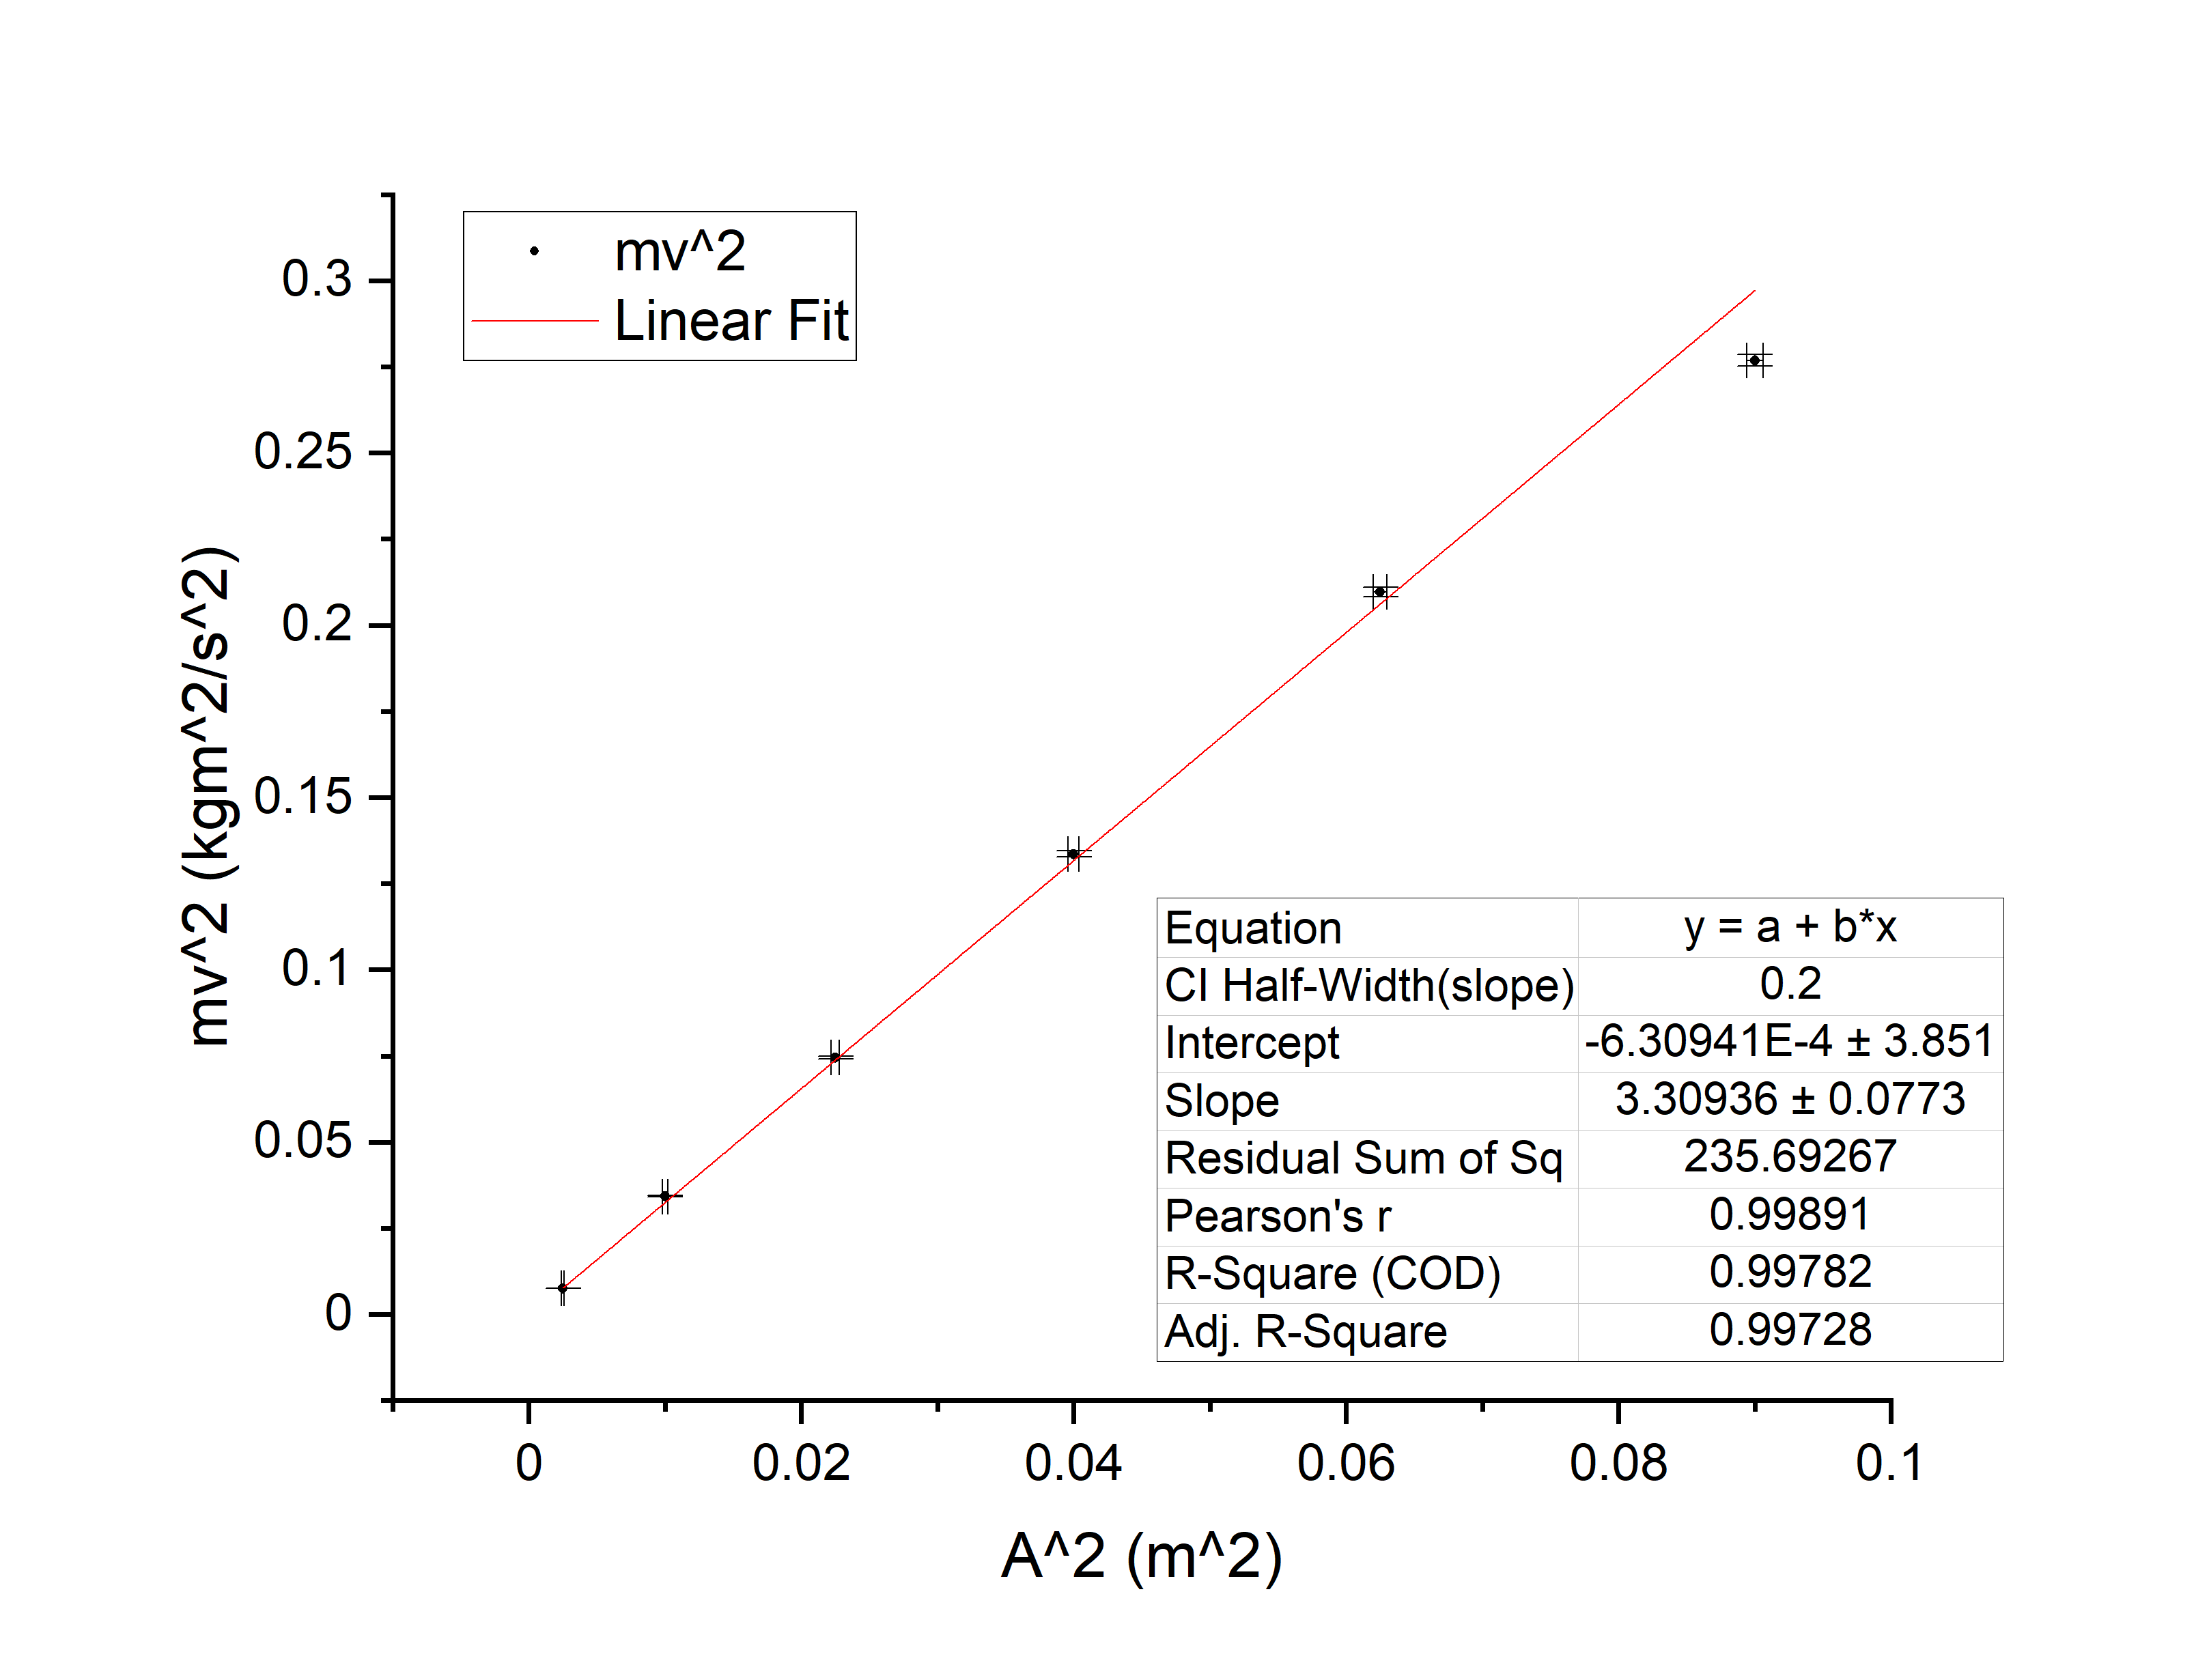
\includegraphics[scale=0.32]{mvsquare.png}
    \caption{$mv^2$ vs. $A^2$}
    \label{mva}
\end{figure}

The total mass equals $M_o+m_4=0.156487\pm0.000015kg$. \par
Then we calculate $m{v_{max}}^2$ and $A^2$. The detailed data is in Table \ref{unceratinyasquare} and \ref{v2maxA}.\par 
From figure, we can get $k1+k2=3.3\pm0.2N/m$, recall 5.2, we find k1+k2=$3.27\pm 0.12N/m$. The relative error is 0.9\%.

\section{Conclusion and Discussion}

\subsection{Conclusions}
In this experiment, we apply the knowledge of Hooke’s law and use the Jolly balance to measure the spring constant. Then we do a series of control experiment to explore the relationship of T\&M, T\&A, Vmax\&A and get the following conclusions:
\begin{itemize}
    \item 	k1= 1.691$\pm$0.015N/m, k2=1.58$\pm$0.12N/m
    \item $T^2$ is directly proportional to M. The inclination of the air track will not affect the slope.
	\item In our measurement range, T and A are almost independent.
	\item M${v_{max}}^2$ is directly proportional to $A^2$.
\end{itemize}

\subsection{Error Analysis}
\begin{itemize}
    \item 	In the measurement of string length, we judged whether three lines coincide with each other before reading. There might exist errors since it’s hard to compare the positions of the three lines. 
    \item Vmax should be measured at the equilibrium position. However, since U-shape shutter has width, we cannot ensure whether the photoelectric gate is fixed at the equilibrium position.
	\item In 5.5, the standard mass of the object should be only the cart and the U-shape shutter. However, we added masses to the cart. Although it does not affect the conclusion, it results in an extra uncertainty factor and increases the uncertainty range.
	\item In the analysis of the relationship between T and A. Although theoretically they are independent, the Pearson’s r is not small enough to indicate this fact. However, the r is affected by the number of trials. We only did 6 trials so that the data seems to fluctuate largely. When the sample size is too small, it is not scientific to determine the correlation between two variables by analyzing r. If we continue to do more trials, the Pearson’s r will be closer to 0 and the result will be clearer. Also, friction has more effect when the amplitude is small. 
	\item In 5.4, the slope of $mv^2$ v.s. $A^2$ is the equivalent spring constant, which is 3.3N/m from the figure. However, the theoretical value of the two springs in parallel is k1+k2=3.27N/m. Our experimental result is bigger, and the error might come from the inaccuracy in the reading of A from the air track.
\end{itemize}

\subsection{Improvement}
\begin{itemize}
    \item When measuring spring constant, uncertainty exists in the step of measuring the weight put on the spring because there is a step multiplying m and g. To increase the accuracy, we can use a forcemeter to replace the mass so that the weight can be directly read.
    \item Use electronic scale to measure the length of springs
    \item Do more trials in section 5.3   
    \item Choose bigger amplitude to reduce the effect of friction
    \item	According to research[1], the effective mass of the spring is not always exactly 1/3 of its mass. When the mass of the object is increased, the error brought by the effective mass can be reduced. Therefore, use a heavier cart might bring more accurate and realistic results.  
\end{itemize}

%----------------------------------------------------------------------------------------
%	DATASHEET
%----------------------------------------------------------------------------------------

\newpage
{\LARGE\textbf{APPENDIX}}
\setcounter{section}{0}
\renewcommand\thesection{\Alph{section}}

\section{Reference}
Qin Tian, Zheng Huan, Li Yingyu, Li Tiantian, Mateusz Krzyzosiak, Vp141, Exercise 3, Simple Harmonic Motion:
Oscillations in Mechanical Systems

\section{Uncertainty Analysis}

\subsection{Uncertainty of the mass $M_0$}
Object with I-shape $m_{obj}=119.18g\pm0.01g=0.11918\pm0.00001kg$\par 
Object with U-shape $m_{obj}=128.34\pm0.01g=0.12834\pm0.00001kg$\par
Mass of spring 1\&2 $m_{spr1\&2}=27.17\pm0.01g=0.02717\pm0.00001kg$\par 
Therefore, we calculate the equivalent mass by $M_o=m_{obj}+\frac{1}{3}m_{spr1\&2}+m_{mass}$\par
For all the M:
$$ \mu_m=\sqrt{\mu_{m_{obj}}^2+\mu_{m_{spr1\&2}}^2\times \frac{1}{3^2}+\mu_{m_{mass}}^2}=\sqrt{0.00001^2\times (1+1+\frac{1}{9})}=1.5\times 10^{-5}kg$$

\subsection{Uncertainty in Measurement of Spring Constant}
\subsubsection{Uncertainty of the weight measurement}
$$w=mg$$
$$\frac{\partial_w}{\partial_m}=g=9.794m/s^2$$
$$\frac{\partial_w}{\partial_g}=m$$
$$u_m=\Delta_A=0.01g$$
$$u_g=0$$
$$u_w=\sqrt{(\frac{\partial_w}{\partial_m})^2{u_m}^2+(\frac{\partial_w}{\partial_g})^2{u_g}^2}=\sqrt{(9.794)^2\times0.00001^2+m^2 \times 0^2}=0.00001N$$
\subsubsection{Uncertainty of the spring deformation measurement}
$$\Delta L=L-L0$$
According to the uncertainty propagation formula,
$$u_{\Delta L}=\sqrt{{u_L}^2\times 2}=\sqrt{0.00002^2\times 2}=0.00003m$$
\subsubsection{Uncertainty of k}
Through the usage of origin, we could find that $u_{k1}=0.015N/m$ and $u_{k2}=0.12N/m$.
$$u_{r,k1}=\frac{0.015}{1.691}=0.89\%$$ 
$$u_{r,k2}=\frac{0.12}{1.58}=7.59\%$$ 

\subsection{Uncertainty in the Analysis of Relation between the Oscillation Period T and the Mass of the Oscillator M}

\subsubsection{Uncertainty of the total mass $M_{tot}$}
$$M_{tot}=M_0+m$$
$$u_{M_{tot}}=\sqrt{(1.05\times 10^{-5})^2+(10^{-5})^2}=1.45\times 10^{-5}kg$$

\subsubsection{Uncertainty of one period T}
$$T=\frac{T_{10}}{10}$$
$$u_T=\frac{1}{10}u_{T_{10}}=10^{-5}s$$

\subsubsection{Uncertainty of $T^2$}
$$\frac{\partial T^2}{\partial T}=2T$$
$$u_T^2=\sqrt{(\frac{\partial T^2}{\partial T})^2{u_T}^2}=\sqrt{4T^2\times (10^{-5}s)^2}=2\times 10^{-5}T$$
All the uncertainty for $T^2$ are listed in the Table \ref{Tsquare}.

\begin{table}[H]
    \centering
    \begin{tabular}{|c|c|c|c|c|c|}\hline
    \multicolumn{6}{|c|}{Uncertainty of $T^2$[$s^2$]}\\\hline 
    \multicolumn{2}{|c|}{horizontal}&\multicolumn{2}{c|}{incline 1}&\multicolumn{2}{c|}{incline 2}\\\hline
    $m_1$&0.00002 &$m_1$& 0.00002 & $m_1$&0.00002 \\\hline
    $m_2$&0.00003 & $m_2$&0.00003 & $m_2$&0.00003 \\\hline
    $m_3$&0.00003 &$m_3$& 0.00003 & $m_3$&0.00003 \\\hline
    $m_4$&0.00003 & $m_4$&0.00003 & $m_4$&0.00003 \\\hline
    $m_5$&0.00003 & $m_5$&0.00003 & $m_5$&0.00003 \\\hline
    $m_6$&0.00003 & $m_6$&0.00003 & $m_6$&0.00003\\\hline
    \end{tabular}
    \caption{Uncertainty of $T^2$}
    \label{Tsquare}
\end{table}

\subsubsection{Uncertainty of theoratical $\frac{T^2}{m}$}

$$\frac{T^2}{m}=4\pi^2\frac{1}{k_1+k_2}$$

\begin{equation*}
    \begin{split}
        \mu_{T^2/m}&=\sqrt{\left(\frac{\partial \frac{4\pi^2}{k_1+k_2}}{\partial k_1}\right)^2\cdot \mu_{k_1}^2+\left(\frac{\partial \frac{4\pi^2}{k_1+k_2}}{\partial k_2}\right)^2\cdot \mu_{k_2}^2}\\
        &=\sqrt{\left(\frac{-4\pi^2}{(k_1+k_2)^2}\right)^2\cdot \mu_{k_1}^2+\left(\frac{-4\pi^2}{(k_1+k_2)^2}\right)^2\cdot \mu_{k_2}^2}\\
        &=\sqrt{\left(\frac{-4\pi^2}{(1.681+1.58)^2}\right)^2\cdot 0.03^2+\left(\frac{-4\pi^2}{(1.691+1.58)^2}\right)^2\cdot 0.03^2}\\
        &=0.16s^2/kg
    \end{split}
\end{equation*}

\subsection{ Uncertainty in the Analysis of Relation between the Oscillation Period T and the Mass of the Oscillator M}
In this part, the A has the uncertainty of 0.1cm and $T_{10}$ has the uncertainty of 0.0001s, so $u_T=0.00001s$. 

\subsection{Uncertainty of $\Delta x$}

\subsubsection{Uncertainty of $x_{in}$}
$$\Delta_B=2\times 10^{-5}m$$
$$\overline{x_{in}}=\sum^3_{i=1}x_{in,i}=\frac{4.44mm+4.46mm+4.44mm}{3}=4.45mm$$
n=3,so $\Delta_A=\frac{t_{0.95}}{\sqrt{n}}\sqrt{\frac{1}{n-1}\sum^n{i=1}(x_{in,i}-\overline{x_{in}})^2}=0.04mm$\par 
The total uncertainty is $u_{x_{in}}=\sqrt{{\Delta_A}^2+{\Delta_B}^2}=0.03mm$
$$u_{r}=\frac{u_{x_{in}}}{x_{in}}\times 100\%=9.0\%$$

\subsubsection{Uncertainty of $x_{out}$}
$$\Delta_B=2\times 10^{-5}m$$
$$\overline{x_{out}}=\sum^3_{i=1}x_{in,i}=\frac{15.50mm+15.54mm+15.52mm}{3}=15.52mm$$
n=3,so $\Delta_A=\frac{t_{0.95}}{\sqrt{n}}\sqrt{\frac{1}{n-1}\sum^n{i=1}(x_{in,i}-\overline{x_{in}})^2}=0.05mm$\par 
The total uncertainty is $u_{x_{in}}=\sqrt{{\Delta_A}^2+{\Delta_B}^2}=0.05mm$
$$u_{r}=\frac{u_{x_{in}}}{x_{in}}\times 100\%=0.3\%$$

\subsubsection{Uncertainty of $\Delta x$}
$$\Delta x=\frac{x_{in}+x_{out}}{2}$$
$$\frac{\partial \Delta x}{\partial x_{in}}=\frac{\partial \Delta x}{\partial x_{out}}=\frac{1}{2}$$
$$u_{x_{in}}=0.04mm,~~u_{x_{out}}=0.05mm$$
$$u_{\Delta x}=\sqrt{(\frac{\partial \Delta x}{\partial x_{in}})^2{u_{x_{in}}}^2+(\frac{\partial \Delta x}{\partial x_{out}})^2{u_{x_{out}}}^2}=0.03mm$$
Therefore, $\Delta x=\frac{x_{in}+x_{out}}{2}=9.99\pm0.03mm=0.00999\pm0.00003m$

\subsection{ Uncertainty in the Analysis of Relation between the Maximum Speed and the Amplitude}

\subsubsection{Uncertainty of $A^2$}
$$\frac{\partial A^2}{\partial A}=2A$$
$$u_{A^2}=\sqrt{(2A)^2\times (10^{-3}m)^2}=2\times c10^{-3}A$$
\begin{table}[H]
    \centering
        \begin{tabular}{|c|c|c|}
            \hline
          A[m]$\pm$0.001[m]  & $A^2$ &   $\mu_{A^2}[m^2]$     \\\hline
        0.0500 & 0.0025& 0.0001 \\\hline
        0.1000 & 0.0100 & 0.0002 \\\hline
        0.1500 & 0.0225 & 0.0003 \\\hline
        0.2000 & 0.0400 & 0.0004 \\\hline
        0.2500 & 0.0625 & 0.0005 \\\hline
        0.3000 & 0.0900 & 0.0006\\\hline
        \end{tabular}
        \caption{Uncertainty for $A^2$}
        \label{unceratinyasquare}
    \end{table}

\subsubsection{Uncertainty of $v_{max}$}
$$v_{max}=\frac{\Delta x}{\Delta t}$$
$$\frac{\partial v_{max}}{\partial \Delta x}=\frac{1}{\Delta t}$$
$$\frac{\partial v_{max}}{\partial \Delta t}=\frac{-\Delta x}{(\Delta t)^2}$$
$$u_{v_{max}}=\sqrt{(\frac{\partial v_{max}}{\partial \Delta x})^2{u_{\Delta x}}^2+(\frac{\partial v_{max}}{\partial \Delta t})^2{u_{\Delta t}}^2}=\sqrt{\frac{(0.00003)^2}{(\Delta t)^2}+\frac{(0.00999*0.00001)^2}{\Delta t^4}}$$
\begin{table}[H]
    \centering
    \begin{tabular}{|c|c|}\hline
    $A[m]\pm 0.001[m]$& $\mu_v[m/s]$\\\hline
    0.050 & 0.0006 \\\hline
    0.100 & 0.0014 \\\hline
    0.150 & 0.002  \\\hline
    0.200 & 0.003  \\\hline
    0.250 & 0.004  \\\hline
    0.300 & 0.004 \\\hline
    \end{tabular}
    \caption{Uncertainty for $v_{max}$}
    \label{uncertaintyvmax}
\end{table}

\subsubsection{Uncertainty of $m{v_{max}}^2$}
$$\frac{\partial m{v_{max}}^2}{\partial m}={v_max}^2$$
$$\frac{\partial m{v_{max}}^2}{\partial v_{max}}=2mv_{max}$$
\begin{equation*}
    \begin{split}
        u_{m{v_{max}}^2}&=\sqrt{(\frac{\partial m{v_{max}}^2}{\partial m})^2{u_m}^2+(\frac{\partial m{v_{max}}^2}{\partial v_{max}})^2{u_{v_{max}}}^2}\\
        &=\sqrt{{v_{max}}^4\times 0.000015^2+(2\times 0.156487\times {v_{max}}^2)\times {u_{v_{max}}}^2}
    \end{split}
\end{equation*}

\begin{table}[H]
    \centering
    \begin{tabular}{|c|c|c|c|c|c|}
    \hline
    $v$[m/s]    & $\mu_v$[m/s] & $m$ [kg] & $\mu_m$[kg]  & $mv^2[kgm^2/s^2]$ & $\mu_{mv^2}[kgm^2/s^2]$ \\ \hline
    0.2200 & 0.0006  & 0.156487 & 0.000015 & 0.00757 & 0.00004      \\ \hline
    0.4673 & 0.0014  & 0.156487 & 0.000015 & 0.0342  & 0.0002       \\ \hline
    0.690  & 0.002   & 0.156487 & 0.000015 & 0.0746  & 0.0004       \\ \hline
    0.924  & 0.003   & 0.156487 & 0.000015 & 0.1336  & 0.0009       \\ \hline
    1.158  & 0.004   & 0.156487 & 0.000015 & 0.2097  & 0.0014       \\ \hline
    1.330  & 0.004   & 0.156487 & 0.000015 & 0.2769  & 0.0017       \\ \hline
    \end{tabular}
    \caption{Data for relation between ${v_max}^2$ v.s. $A$}
    \label{v2maxA}
\end{table}

\section{Implementary figures}
\begin{figure}[H]
    \centering
        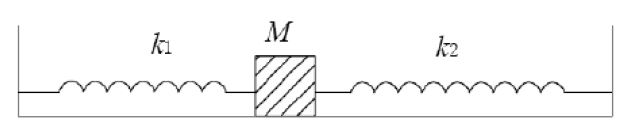
\includegraphics[width=13cm]{figure1.png}
        \caption{Mass-spring system}
        \label{masssystem}
\end{figure}

\begin{figure}[H]
    \centering
    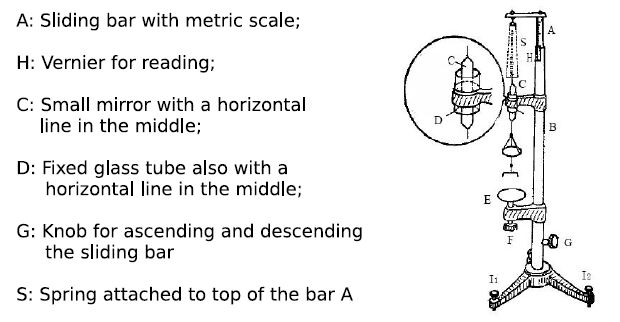
\includegraphics[width=12cm]{jollybalance.png}
    \caption{Jolly Balance}
    \label{jolly}
\end{figure}

\begin{figure}[H]
    \centering
    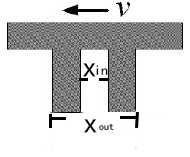
\includegraphics[width=5cm]{ushape.png}
    \caption{the U-shape shutter}
    \label{ushape}
\end{figure}

\begin{figure}[H]
    \centering
    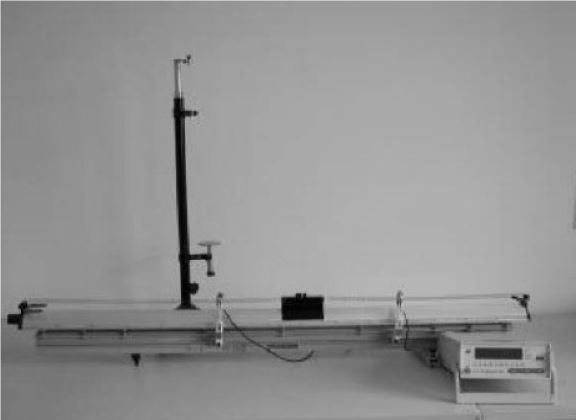
\includegraphics[width=12cm]{setup.png}
    \caption{the experimental setup}
    \label{setup}
\end{figure}

\section{Implementary tables}
\begin{table}[H]
    \centering
    \begin{tabular}{|c|c|c|}
    \hline
      & m{[}kg{]}$\pm10^{-5}${[}kg{]} & w{[}N{]}$\pm10^{-5}${[}N{]} \\ \hline
    1 & 0.00479 & 0.04691         \\ \hline
    2 & 0.00950 & 0.09304         \\ \hline
    3 & 0.01426 & 0.13966         \\ \hline
    4 & 0.01909 & 0.18697         \\ \hline
    5 & 0.02390 & 0.23408         \\ \hline
    6 & 0.02863 & 0.28040         \\ \hline
    \end{tabular}
    \caption{Weight Measurement Data}
    \label{weight}
\end{table}

\begin{table}[H]
    \centering
    \begin{tabular}{|c|c|c|c|c|}
    \hline
       & \multicolumn{2}{c|}{Spring1}         & \multicolumn{2}{c|}{Spring2}         \\ \hline
       & L{[}mm{]}$\pm$0.02{[}mm{]} & $\Delta$L{[}mm{]}$\pm$0.02{[}mm{]} & L{[}mm{]}$\pm$0.02{[}mm{]} & $\Delta$L{[}mm{]}$\pm$0.02{[}mm{]} \\ \hline
    L  & \multicolumn{2}{c|}{360.60}& \multicolumn{2}{c|}{360.54}\\ \hline
    L1 & 389.54      & 28.94       & 388.30       & 27.76       \\ \hline
    L2 & 416.62      & 56.02       & 415.78      & 65.24       \\ \hline
    L3 & 444.46      & 83.86       & 444.24      & 93.70        \\ \hline
    L4 & 471.76      & 111.16      & 472.14      & 121.60       \\ \hline
    L5 & 500.08      & 139.48      & 500.16      & 149.62      \\ \hline
    L6 & 527.68      & 167.08      & 528.80       & 178.26      \\ \hline
    \end{tabular}
    \caption{$\Delta$L measurement data}
    \label{deltal}
 \end{table}

 
\begin{table}[H]
    \centering
    \begin{tabular}{|c|c|c|c|}
    \hline
    \multirow{2}{*}{m[kg]} & \multicolumn{3}{c|}{$T^2$[$s^2$]}            \\ \cline{2-4} 
                       & horizontal & incline 1 & incline2 \\ \hline
    0.13303            & 1.5428     & 1.5436    & 1.5427   \\ \hline
    0.13774            & 1.5964     & 1.5964    & 1.5977   \\ \hline
    0.14250            & 1.6528     & 1.6531    & 1.6531   \\ \hline
    0.14733            & 1.7082     & 1.7105    & 1.7090   \\ \hline
    0.15214            & 1.7643     & 1.7647    & 1.7652   \\ \hline
    0.15687            & 1.8201     & 1.8187    & 1.8207   \\ \hline
    \end{tabular}
    \caption{T square and Mass Data for T v.s. M relation}
    \label{tsquaretable}
\end{table}

\section{Data Sheet}

\end{document}